 \documentclass[oneside]{book}
\usepackage[latin1]{inputenc}
\inputencoding{utf8}
\usepackage[italian]{babel}
\usepackage{xcolor}

\usepackage{hyperref}
\usepackage{subfigure}
\usepackage{mathtools}

\hypersetup{colorlinks=true, linkcolor=blue}
\newcommand{\mail}[1]{\href{mailto:#1}{\texttt{#1}}}

\title{Appunti IUM}
%\author{\href{https://alexflyce.wordpress.com/}{\textbf{\emph{Alessandro Francucci}}}}
\author{\textbf{\emph{Alessandro Francucci}}}

\begin{document}

\pagenumbering{Roman}
\begin{titlepage}
\maketitle
\thispagestyle{empty}
\end{titlepage}
\pagenumbering{arabic}

\tableofcontents


\chapter*{Introduzione}
	In questo pdf verranno trattati, nella maniera più \emph{descrittiva e strutturata} possibile, gli argomenti trattati a lezione dal prof. Panizzi. \emph{Buona Lettura!}

	\section*{Metodi Di Osservazione}
		Per una \emph{valutazione di un interfaccia}, è necessario dover adoperare varie \emph{tecniche}, (dette appunto di \emph{valutazione}) che ci consentono di avere un feedback sull'interfaccia stessa.\footnote{E che di conseguenza ci permettono di migliorarne il risultato} I principali \emph{step} per una valutazione \emph{efficiente}, possono essere riassunti con:
		\begin{enumerate}
			\item Test dell'\emph{usabilità} e delle \emph{funzionalità} del sistema
			\item Prove in laboratorio e sul campo con gli utenti
			\item Valutando sia la progettazione che l'implementazione
			\item Considerando tutti i vari cicli di vita nella progettazione
		\end{enumerate}
		Tra gli obbiettivi più importanti di queste \emph{valutazioni}, è bene sottolineare il fatto che quest'ultime ci consentono di:
		\begin{enumerate}
			\item Valutare l'\emph{estendibilità} delle funzioni di un sistema
			\item Valutare gli \emph{effetti} dell'interfaccia sull'\emph{utente}
			\item Identificare determinati \emph{problemi specifici}
		\end{enumerate}
		Detto questo, non ci resta che addentrarci nelle varie \emph{tecniche di valutazione}.



\chapter{Tecniche di Valutazione}  
	Le \emph{tecniche di valutazione} (precedentemente accennate) che vengono utilizzate e che vedremo, si distinguono in 3 grandi categorie. Ovvero in quelle:
	\begin{enumerate}
		\item Basate sull'\emph{utente}
		\item Basate su \emph{esperti}
		\item Basate sull'\emph{interrogazione}\footnote{ Le tecniche di valutazione basate sull'interrogazione, quali \emph{interviste} e \emph{questionari}, verranno discusse solamente per quel che riguarda il \emph{Needfinding}, ovvero un argomento molto importante del prossimo capitolo. (\ref{sec:Needfinding})} 
	\end{enumerate}
	Prima di iniziare descrivendo nel dettaglio il primo approccio, di seguito è possibile osservare una tabella che riassume brevemente i principali concetti di queste 3 categorie:
	\begin{figure}[h] \label{fig:schemaTecnicheVal}
		\centering%
		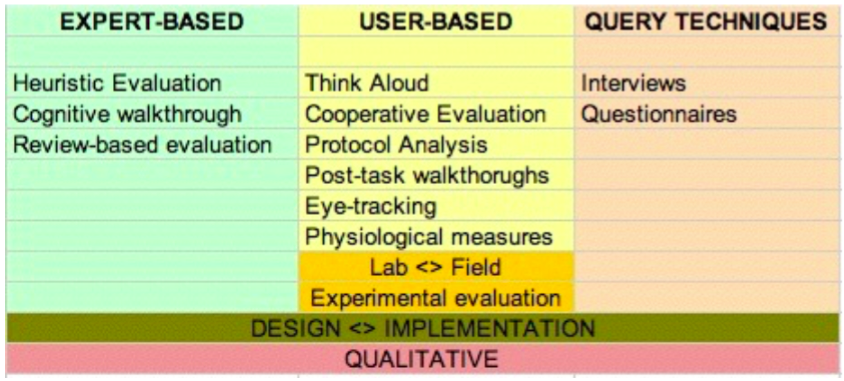
\includegraphics[height = 48mm]{images/schema.png}
	\end{figure}

	\section{Valutazione con Participazione Utente} 
		Per quanto riguarda questo primo tipo di \emph{valutazione}, è opportuno che si distinguino i due approcci fondamentali, ovvero quello in \emph{laboratorio} e quello sul \emph{campo}.
		
		\subsection{Laboratorio} \label{sec:laboratoriocampo}
			I vantaggi di effettuare delle valutazioni attraverso la partecipazione degli utenti in laboratorio, possono essere notevoli. Possiamo infatti godere di:
			\begin{itemize}
			\item \emph{Ambiente non interrotto} (ovvero senza disturbo)
			\item Materiale specializzato 
			\end{itemize}
			D'altro canto, tra gli svantaggi di questo approccio emerge la:
			\begin{itemize}
			\item \emph{Perdita di contesto}
			\item Difficoltà nell'osservare diversi utenti che cooperano
			\end{itemize}
			È importante sottolineare però che per determinate app è impossibile adottare un approccio \emph{diverso} da quello in laboratorio. Per capire il \emph{perché} di quanto detto, basta descrivere pregi e difetti anche dell'altro approccio, ovvero quello sul \emph{campo}.

		\subsection{Campo}
			Il ``contendente'' all'approccio in laboratorio, è quello sul \emph{campo}, che permette di effettuare i \emph{test} in \emph{prossimità dell'utente}.\\ 
			\\ \textbf{Vantaggi}:
			\begin{itemize}
			\item \emph{Naturalezza} (Non ci sono tutte quelle ``pressioni'' che l'utente poteva avvertire come nel laboratorio)
			\item \emph{Contesto mantenuto} (L'applicazione viene provata in uno scenario non troppo diverso da quello reale)
			\item Possibilità di \emph{studi longitudinali} (A distanza di giorni, mesi, anni)
			\end{itemize}
			Tra gli svantaggi invece va evidenziato il fatto che sul campo possono esserci più \emph{distrazioni}, rumori e via dicendo.. Tuttavia, questo approccio è particolarmente indicato quando il contesto si rileva essere \emph{cruciale}.\footnote{NB: Come detto nella sezione \ref{sec:laboratoriocampo}, a volte non è possibile attuare l'approccio sul \emph{campo}. Perché? Basti pensare ad app con un contesto d'uso non pratico. Es: Utility Aerospaziale, (l'ho sparata grossa, ma rende l'idea) etc.}

		\subsection{Metodi di osservazione} \label{MetodiDiOsservazione}
			Abbiamo appena descritto i vari approcci possibili sul \textbf{\emph{dove}} sia meglio operare. Adesso è opportuno descrivere anche i vari \emph{metodi} che dobbiamo usare per le nostre \emph{valutazioni}. \\
			Prima di vederli, è importante precisare i due \emph{ruoli} fondamentali di coloro che effettueranno la valutazione, che sono rispettivamente \emph{l'administrator} (che in genere è colui che porge le domande/interagisce con l'utente) e \emph{l'observer} (ovvero colui che prende nota dei risultati ottenuti dai vari test). Vediamo adesso questi metodi nel dettaglio:

			\subsubsection{Think Aloud}
				il ``think aloud'' (pensare ad alta voce), è uno dei metodi più semplici e, per tal ragione, più usati per la valutazione di un interfaccia. \\

				\textbf{\emph{Come Funziona}}: Quando si fa il test, si chiede all'utente di dire ad alta voce quello che sta pensando / facendo. \\

				\textbf{\emph{A Cosa Serve?}} Serve a farsi un idea di cosa sta facendo l'utente. Ha il vantaggio inoltre di essere semplice, ed è fattibile anche dal punto di vista dell'utente, visto che chiunque è in grado di dire cosa sta facendo.\\

				\textbf{\emph{Svantaggi}}: Il fatto stesso di pensare ad alta voce, fa cambiare il comportamento ``naturale'' delle persone. Inoltre, i risultati ottenuti secondo questo approccio (dove l'utente non è praticamente guidato) sono molto soggettivi.

			\subsubsection{Cooperative Evaluation}
				La Valutazione Cooperativa, è una variante dell'approccio del metodo precedentemente descritto. \\

				\textbf{\emph{Come Funziona}}: Anche qui, viene chiesto all'utente di eseguire i task ad alta voce, ma stavolta c'è \emph{interazione} tra l'utente e l'amministratore. L'utente infatti può chiedere ciò che vuole all'amministratore. \\

				\textbf{\emph{Vantaggi}}: Tra i vantaggi di questo metodo, oltre a quelli del ``think aloud'', che in un certo senso sono ``ereditati'', bisogna sottolineare il fatto che adesso l'utente è \emph{incoraggiato} a criticare eventualmente il sistema, (grazie all'amministratore) e che il sistema risulti più chiaro da parte di chi lo usa. \\

				\textbf{\emph{Svantaggi}}: Nonostante ci sia meno tensione da parte dell'utente, grazie al dialogo con l'amministratore, abbiamo anche lo svantaggio che la presenza dell'admin cambia le azioni dell'utente. (visto che può fare domande, al momento del test non farà errori che magari in altre circostanze avrebbe commesso)

			\subsubsection{Protocol Analysis}
				L'analisi di protocollo, è una variante che si diversifica su più aspetti dai metodi presentati finora. \\

				\textbf{\emph{Come Funziona}}: \emph{L'analisi di protocollo} ha la caratteristica che, quando si fanno eseguire i vari task all'utente, si registra qualsiasi azione da esso compiuto.\\

				\textbf{\emph{Vantaggi}}: Permette di avere una accuratezza indiscutibile su quanto fatto dall'utente, riesaminabile anche in un secondo momento. \\

				\textbf{\emph{Svantaggi}}: Richiede attrezzatura adeguata per registrare sia l'audio che il video, nonché una quantità eccessiva di tempo per rivedere le eventuali registrazioni. Soluzioni? Si adotta un \emph{Mixed-use}, ovvero una via di mezzo tra la registrazione completa e gli appunti dell'observer.				

			\subsubsection{Post-Task Walkthroughs}
				Anche questo metodo, prende spunto in un certo senso dal metodo precedente. Vediamo il perchè. \\

				\textbf{\emph{Come Funziona}}: Anche qui, si registra qualsiasi cosa viene fatta dall'utente, esattamente come il metodo precedente, ma a differenza di quest'ultimo, il tutto viene poi fatto rivedere all'utente stesso in modo da poter comprendere meglio determinate scelte. \\

				In questo caso però, bisogna poi seguire una di due diverse procedure, che dipendono strettamente dal momento in cui vengono poste le domande agli utenti:
				\begin{description}
				\item[Immediato] Se le domande vengono fatte subito dopo che l'utente ha eseguito i task, si ha il vantaggio che l'utente è ``fresco'', ovvero ricorda perfettamente il perché di determinate azioni.
				\item[Prolungato] Se le domande vengono invece fatte dopo un certo tempo, abbiamo lo svantaggio che l'utente potrebbe non ricordare il perché di determinate azioni, ma il vantaggio che i valutatori hanno il tempo di formulare al meglio le domande e farsi spiegare in maniera dettagliata la scelta di determinate azioni, magari non comprese.
				\end{description}

				È bene infine sottolineare e ricordare che la \emph{valutazione} del software, cambia significativamente la \emph{qualità} di esso. 

				\pagebreak

	\section{Valutazione Dell'implementazione}
		In questa seconda sezione, discuteremo la cosidetta ``progettazione dell'esperimento'', ovvero un argomento che, pur non costituendo una vera e propria ``tecnica di valutazione''\footnote{ Per avere un quadro delle \emph{tecniche di valutazione}, si riveda sempre la tabella di inizio capitolo. (\ref{fig:schemaTecnicheVal})}, ci fornisce alcuni concetti inerenti agli \emph{esperimenti} molti importanti. Vediamoli dunque nel dettaglio.

		\subsection{Valutazioni Sperimentali}
			Le valutazioni sperimentali consistono in \emph{valutazioni controllate} di specifici aspetti del \emph{comportamento interattivo}. Quello che il \emph{valutatore} deve fare principalmente in queste valutazioni, è scegliere l'\emph{ipotesi} da testare. Solitamente quello che avviene in queste valutazioni, è il test di diversi esperimenti su una stessa interfaccia, con cambiamenti in poche variabili controllate. \\


		\subsection{Fattori sperimentali}
			I fattori sperimentali, possono essere semplicemente riassunti in 4 concetti fondamentali:
			\begin{description}
			\item[Soggetto] \emph{Chi} rappresenta l'azione
			\item[Variabili] Oggetti da modificare e misurare
			\item[Ipotesi] Cosa si vuole mostrare
			\item[Progettazione sperimentale] Come si è intenzionati a procedere
			\end{description}
			Elencati i concetti, addentriamoci ulteriormente in alcuni di essi.

			\subsubsection{Variabili}
				Le Variabili si distinguono in due categorie.
				\begin{description}
				\item[Variabili Indipendenti (IV)] Ovvero quelle indipendenti dal soggetto, e che quindi possiamo cambiare. (come per esempio alcuni bottoni, menù e via dicendo..)
				\item[Variabili Dipendenti (DV)] Ovvero quelle che riguardano tutte le caratteristiche \emph{misurabili} durante l'esperimento. (Come il tempo impiegato dall'utente per eseguire una task particolare, o il numero di errori da lui commesso) \emph{Non possiamo agire direttamente su questo tipo di variabili.}
				\end{description}

			\subsubsection{Ipotesi}
				Le \emph{ipotesi} altro non sono che una predizione del risultato, in termini delle variabili \emph{dipendenti} e \emph{indipendenti}.\footnote{ \textbf{Esempio Ipotesi}: \emph{``L'errore è proporziale alla grandezza del font.''}} 
				\begin{description}
				\item[Ipotesi Nulla] Si tratta di una contro ipotesi da confutare. (Es: Al variare della dimensione del bottone, i tempi totali non varieranno.)
				\end{description}

		\subsection{Design Sperimentale} \label{sez:wbgroups}
			Quando devo far fare diversi test agli utenti, magari tra alcune interfacce che presentano cambiamenti minimi (come le dimensioni o la posizione di un bottone etc.) esistono vari approcci possibili. Ovvero:
			\begin{description}
			\item[Within Groups] Dove ogni soggetto esegue l'esperimento \emph{sotto le varie condizioni}.
			\item[Between Groups] Dove ogni soggetto esegue la sua azione su \textbf{una sola} condizione.
			\end{description}
			\begin{em}
			\begin{center}
			Quali sono dunque i vantaggi e gli svantaggi? 
			\end{center}
			\end{em}
			Per quanto riguarda il \emph{within groups} bisogna dire che, se da una parte ho il grando vantaggio di avere un \emph{maggior numero di test a parità di utenti}, dall'altra ho lo svantaggio che i test sono \emph{condizionati} dall'apprendimento da parte dell'utente.\footnote{\textbf{Osservazione Personale}: Alcune volte, nei test \emph{within groups}, può essere interessante chiedere all'utente di esprimere una preferenza sulle interfacce provate. Fare ciò, non è utile per la semplice risposta in sè, (che potrebbe essere in alcuni casi poco oggettiva) ma lo è per via del \emph{perché}, che potrebbe portarci ad osservazioni non cosiderate o nuovi punti di vista.
			}
			Infatti, come è intuitivamente possibile immaginare, se tra i vari test i cambiamenti sono minimi, l'utente nei test successivi al primo esiterà decisamente di meno sul da farsi.

			Il between groups invece, richiede semplicemente una maggiore quantità di tempo per trovare gli utenti. \\

			\textbf{Attenzione!} Nei test come questo, è importante anche la \emph{selezione degli utenti}, in quanto le \emph{skill} di un utente, influenzano pesantemente la prova.\footnote{ Se per esempio voglio vedere se è meglio usare un bottone di 1cm per la registrazione su un sito oppure uno da 3, la prova mi può portare a soluzioni non valide qualora il primo test la faccio fare a persone con esperienza nel settore informatico, mentre il secondo alla celeberrima \emph{``confraternita del vecchio saggio''.}} È bene dunque scegliere opportunamente i soggetti rappresentanti! (ovvero è necessario che appartengano tutti alla stessa \emph{classe}, dove per classe intendiamo persone della stessa età e con un campo di conoscenze simili).

			\pagebreak

	\section{Expert Based} \label{sec:expertBased}
		Ultimo ed interessante approccio, per quanto riguarda le \emph{tecniche di valutazione}, è quello \emph{basato sugli esperti}. Questo tipo di valutazione, si basa su tre concetti cardine, che esamineremo singolarmente. 

		\subsection{Cognitive Walkthrough}
			Questo approccio è eseguito molto spesso da esperti in psicologia. Bisogna infatti capire \emph{cosa apprende} effettivamente l'utente al termine di ogni task. (se trae soddisfazione dalle azioni compiute oppure no) \\
			La domanda principale da porci dunque è\dots \emph{L'interfaccia porta l'utente al raggiungimento dei sperati obbiettivi?} \\

			In sostanza, grazie ai principi della psicologia, si riescono ad identificare gli eventuali problemi dell'interfaccia.

		\subsection{Heuristic Evaluation} \label{sec:heuristic}
			La valutazione eulistica, (che dobbiamo a \emph{Nielsen}) è probabilmente il metodo migliore tra quelli elencati. \emph{Come funziona questo metodo?} Si basa ``semplicemente'' sulla verifica di 10 criteri, che non sono però immediati da capire. Vediamoli adesso nel dettaglio.\footnote{ Vengono elencati per completezza. Non è necessario studiarli nel dettaglio ai fini dell'orale.}
			\begin{enumerate}

			\item \textbf{Informare l’utente sullo stato del sistema} \\
			Il sistema deve sempre tenere informato l’utente su cosa sta facendo, fornendo un adeguato feedback in un tempo ragionevole. \\
			\emph{Esempi e Domande Lecite}: 

			Presenza di un segnale di attività in corso (clessidra, barra di caricamento, messaggio testuale, etc.) \\
			Icona o testo \textcolor{gray}{sotto-intensificato}. (indica che la funzione non è disponibile) \\
			Cosa sta facendo il sistema? \\
			Dove mi trovo rispetto all’interazione avuta col sistema? \\
			Che effetto ha avuto o sta avendo la mia azione? \\

			\item \textbf{Corrispondenza tra sistema e mondo reale} \\
			Il sistema deve parlare il linguaggio dell’utente, con parole, frasi e concetti a lui familiari. \\
			\emph{Esempi e Domande Lecite}: 

			Uso di messaggi testuali, icone, azioni dal significato condiviso da tutti (``salva con nome'', azione ``copia e incolla'')\\
			Non mostrare all’utente la terminologia propria del sistema \\

			\item \textbf{Controllo e libertà} \\
			L’utente deve avere il controllo del contenuto informativo e muoversi liberamente tra i vari argomenti.\\
			\emph{Esempi e Domande Lecite}: 

			Evitare procedure costrittive troppo lunghe (iscrizioni) \\
			Evitare percorsi predefiniti senza possibili scorciatoie \\
			Evitare azioni non volute dall’utente (apertura automatica di pagine non richieste) \\
			Fare in modo che l’utente non si senta in trappola \\

			\item \textbf{Consistenza e standard} \\
			L’utente deve aspettarsi che le convenzioni del sistema siano valide per tutta l’interfaccia. \\
			\emph{Esempi e Domande Lecite}: 

			Riportare in ogni pagina alcuni elementi di riconoscimento (logo, stile grafico, etc.) \\
			Dare la sensazione di essere sempre nello stesso ambiente\\

			\item \textbf{Prevenzione dell’errore} \\
			Evitare di porre l’utente in situazione ambigue, critiche e che possono portare all’errore.\\
			\emph{Esempi e Domande Lecite}: 

			Dare la possibilità di tornare indietro \\
			Evitare che la non comprensione induca in errore \\

			\item \textbf{Riconoscimento anziché ricordo} \\
			Le istruzioni per l’uso del sistema devono essere ben visibili e facilmente recuperabili.\\
			\emph{Esempi e Domande Lecite}: 


			Produrre layout semplici e schematici \\
			Non contare sulla capacità dell’utente di ricordare il posizionamento degli oggetti che caratterizzano le pagine \\
			Evitare che l’utente riscopra ogni volta l’interfaccia \\

						\item \textbf{Flessibilità d’uso} \\
			Offrire all’utente la possibilità di un uso differenziale (a seconda della sua esperienza) dell’interfaccia. \\
			\emph{Esempi e Domande Lecite}: 
			Consentire agli utenti più esperti di fare le azioni più frequenti nel modo più veloce. \\
			Offrire una navigazione gerarchica per i meno esperti \\

			\item \textbf{Design e estetica minimalista} \\
			Dare maggior importanza al contenuto che all’estetica. \\
			\emph{Esempi e Domande Lecite}: 
			Evitare di accentuare oggetti irrilevanti o raramente necessari (immagini grandi, etc.) \\
			Evitare che il contenuto informativo della pagina sia messo in secondo piano \\
			Evitare che l’utente si distragga o si confonda \\

			\item \textbf{Aiuto all’utente} \\
			Aiutare l’utente a riconoscere, diagnosticare e recuperare l’errore. \\
			\emph{Esempi e Domande Lecite}: 
			I messaggi di errore devono essere espressi in linguaggio comprensibile (senza codici) \\
			I messaggi di errore devono indicare in modo preciso il problema e suggerire una soluzione \\
			Chiedere conferma per un’azione importante \\

			\item \textbf{Documentazione} \\
			Anche se il sistema dovrebbe essere usabile senza documentazione è preferibile che essa sia disponibile \\
			\emph{Esempi e Domande Lecite}: 
			Deve essere facile da reperire \\
			Focalizzata sul compito dell’utente \\
			Strutturata in un insieme di passi comprensibili \\
			\end{enumerate}

		\subsection{Review Based Evaluation} \label{reviewbasedevaluation}
			La \emph{review based evaluation} invece, è un altro metodo di valutazione che si basa su \emph{risultati sperimentali} e prove \emph{empiriche} della letteratura, in modo tale da rifiutare o accettare parte della progettazione dell'interfaccia.



\chapter{Progetto e sviluppo di sistemi Interattivi}

	\emph{Cosa è il design?} \\È il raggiungimento di determinati obbiettivi, tenendo conto dei \emph{vincoli}. (legati al materiale, alle piattaforme etc.) \\\\
	Che differenza c'è allora tra un \emph{designer} e un \emph{artista}? \\
	L'artista non si interessa se quello che fa, piace o meno al pubblico, in quanto esprime se stesso in ciò che produce. Il \emph{designer} invece, è fortemente vincolato dal suo pubblico! Bisogna chiedersi se quello che facciamo è versatile, utilizzabile e comprensibile.

	Il designer deve perciò basarsi su dei \emph{trade offs} (compromessi), lavorando spesso in gruppo.\footnote{Ciò implica che si devono mettere insieme esperienze differenti.} \\\\
	\emph{Cosa fanno i designer?} \\ Scelgono tecniche, (linguaggi,template, piattaforme etc) sperimentano, tengono conto della ``componente psicologica'' e dei \emph{costi}.

	Detto ciò, è bene notare che il design\footnote{ Design è una parola che abbiamo avuto modo di utilizzare più volte fino adesso, che dall'inglese fa riferimento al concetto di ``progettazione''.} non è \textbf{mai completo}! È in continua evoluzione, e quindi necessita di dover mettere dei ``punti''. (ovvero quelli che noi chiamiamo più semplicemente ``rilasci'') \\

	Vediamo adesso le principali regole per un designer:
	\begin{enumerate}
	\item Sapere come funzionano i computer. (non solo in linea teorica)
	\item Capire le persone. (di cosa hanno effettivamente bisogno)
	\item Capire l'interazione tra il computer e utenti
	\end{enumerate}
	Le regole precedentemente elencate, servono per farci arrivare al nostro \emph{goal}, che consiste nel raggiungimento di \emph{progetti} che godono di un ottima \emph{usabilità}\footnote{ Dove per usabilità (o facilità d'uso) intendiamo un progetto che rispetti 3 caratteristiche fondamentali, ovvero: \emph{l'efficacia, l'efficenza e la soddisfazione}. È di fondamentale importanza inoltre che questo concetto sia considerato \emph{ad ogni passo} nella realizzazione del software, e \textbf{non} solo alla fine!} \\
	
	Fatte queste premesse, andiamo a vedere uno dei modelli più famosi per la progettazione del \emph{software}, (anche se di cattivo esempio per un designer) ovvero il \emph{modello a cascata}.

	\section{Modello a Cascata} \label{sec:Cascata}
		Il modello a cascata si basa su una serie \emph{sequenziale} di passi:
		\begin{itemize}
		\item Requisiti
		\item Progetto architetturale
		\item Progetto dettagliato
		\item Coding fino al testing
		\item Integrazione e testing
		\item Manutenzione
		\end{itemize}
		Fino a una quindicina di anni fa, questo modello era largamente utilizzato, tanto è vero che ogni modulo era associato a gruppi diversi di persone. Nonostante questo, il modello non è particolarmente conveniente per un designer. Per vedere la cosa al meglio, mostriamo un confronto con \emph{l'Ingegneria civile}. \\

		\emph{Procedimento Ing:} Gli ingegneri, prima di progettare un edificio, devono fare un disegno con ogni specifica del palazzo. Dopo la fase di progetto, si passerà la \emph{specifica realizzativa} all'ente adeguato. \\
		Per quanto riguarda i costi però, è bene notare che quest'ultimi sono impiegati maggiormente per la \emph{parte pratica}! (con un bel 90\% circa) Solo la parte rimanente è destinata al designer. \\

		Per quanto riguarda il software invece, è molto difficile parlare di \emph{progetto e sviluppo} in modo separato (contrariamente a quanto avviene nell'esempio precedente). Una cosa molto importante infatti durante la progettazione, è la \emph{visibilità} che si ha del sistema. \\

		Il sistema a cascata di conseguenza, non è particolarmente efficiente in molti casi. Un primo problema di fallimento è il \emph{tempo}. Questa variabile ha infatti un peso particolare in informatica, dove tutto è in continua evoluzione.
		
		\newpage

		Altri fattori sono invece:
		\begin{itemize}
			\item  I Requisiti iniziali sono incompleti, visto che all'inizio nessuno probabilmente ha chiaro cosa bisogna fare.
			\item Gli utenti mi danno dei feedback che mi spingono a fare scelte diverse, spingendomi così a modificare moduli di lavoro magari già terminati.
			\item Durante la realizzazione, riesco a scovare alcuni aspetti che non avevo compreso perfettamente in una prima analisi.. (cosa analoga al primo punto) e così via.
		\end{itemize}
		Il progetto software è meglio dunque se è di \emph{tipo iterativo} (come il prossimo modello che vedremo) piuttosto che di tipo \emph{sequenziale}. \\

		\begin{em}
		\small{\textbf{Morale}: É praticamente indispensabile dover perdere quella tanto amata linearità che avevamo nel modello appena proposto, se vogliamo progettare un software di un buon livello.}
		\end{em}

	\section{Modello Agile}
		Un altro modo di gestire il progetto, è il modello agile che vanta le seguenti caratteristiche:
		\begin{enumerate}
		\item Controllo frequente
		\item Capacità di adattarsi
		\item Incoraggia il modo di lavorare in gruppo 
		\item Possibilità di rilasciare rapidamente software funzionante
		\item Allinearsi alle richieste dei clienti
		\end{enumerate}
		Già da queste fondamentali linee di principio possiamo vedere che ci sono molte differenze tra questo modello e quello a cascata. Nel modello a cascata non c'è molta possibilità di \emph{adattarsi}, (contrariamente a questo modello, che ne fa un punto forte) e la dove gli errori erano difficili da scovare e mi comportavano una grande perdita di lavoro, qui si riesce a scovare quest'ultimi molto più velocemente, consentendomi anche di adattarmi di conseguenza, senza necessariamente apportare chissà quali modifiche. \\

		Un altra differenza sostanziale consiste nel fatto che, mentre il modello a cascata dava enfasi al \emph{processo}, dove nessuno è insostituibile visto che tutto era ``scritto'', il processo agile invece è \emph{people oriented}, ed è importante dunque avere un ambiente sereno nel team, visto che qui le persone non sono facilmente sostituibili.\footnote{ Le persone in questo tipo di approccio sono solitamente \emph{skilled}, ovvero particolarmente intelligenti e dotate per certi compiti.} \\

		In estrema sintesi possiamo inoltre dire che l'\emph{Agile} ``spezzetta'' in più cicli quello che di solito viene fatto in un unico ciclo. Quindi le fasi di \emph{Analisi, Progettazione, Programmazione, QA Testing e Rilascio} vengono svolte solo per un piccolo gruppo di funzionalità, per poi essere ripetute per i cicli che seguono. Ognuna di queste fasi (quasi sempre di carattere incrementale) è chiamato nella terminologia Agile: \emph{sprint}\footnote{ Lo sprint è un unità di base del metodo \emph{Scrum}, che permette di avere una realease funzionale di un software in poco tempo. (Tendenzialmente: 1-4 Settimane)}. (Approfondimenti: \href{https://it.wikipedia.org/wiki/Scrum_(informatica)#Sprint}{\emph{Metodo Scrum}})\\
		
		Altre peculiarità del metodo agile sono:
		\begin{itemize}
		\item \emph{Pair Design Programming}, ovvero una metodologia in cui si programma in due, alternandosi. (uno vede gli errori dell'altro ed eventualmente li corregge) 
		\item \emph{Close Proximity Teams}, dove Team diversi lavorano vicini (fisicamente parlando).
		\end{itemize}

		\subsection{UCD: User-Centered Design} \label{sec:UCD}
			Esiste anche un altro modello iterativo abbastanza vicino all'Agile, ovvero il \emph{modello UCD}, che è decisamente molto più vicino all'utente (Non a caso si chiama User-Centered Design) e cerca di capire di \emph{cosa} quest'ultimo ha effettivamente bisogno. \\
			Da solo però, l'UCD nonostante questo fondamentale pregio, non gode delle fantastiche carrateristiche precedentemente elencate del metodo Agile, (a dir poco fondamentali, come l'early realease, le collaborazioni interdisciplinari tra i dipendenti, lo sprint, il pair design programming etc.) ed è dunque per questo motivo che nasce così il Metodo \emph{Agile UCD}. \\
		
		\subsection{Agile UCD} 
			Questo nuovo modello ``ibrido'', ha dunque il vantaggio che riesce a colmare le principali lacune dei due metodi, come l'\emph{early release} (per l'UCD) e la \emph{vicinanza all'utenza} (per l'Agile). \\
			Per completezza, è bene mostrare allora tutte le fasi principali di questo nuovo metodo.\footnote{La descrizione dettagliata delle fasi è opzionale. Tutto il materiale è stato preso da \href{http://www.progettareperlepersone.it/dblog/articolo.asp?articolo=104}{qui}.}
			\begin{description}
			\item[Fase A - Ricerca e analisi] La fase di Ricerca e analisi è fondamentale per la buona riuscita di un progetto. Oltre a definire gli obiettivi aziendali e gli scopi dell'applicazione, si pianificano le attività di ricerca per acquisire informazioni sui suoi fruitori, potenziali o reali che siano. A tal fine si effettuano interviste all’interno dell’azienda, si analizza la concorrenza etc. Al termine di queste attività il committente deve tassativamente approvare un documento dove sono riportati gli obiettivi del progetto. 

			\item[Fase B - Sprint 0] \emph{Sviluppo dei personaggi, degli scenari e delle stories}: \\
			Servendoci dei risultati delle ricerche possiamo, nello sprint 0, definire i personaggi e gli scenari che ci porteranno a individuare le principali \emph{stories} (altro termine dello sviluppo Agile).\footnote{ Una \emph{User Stories}, potremmo vederla come la descrizione ad alto livello di una funzionalità utile al raggiungimento di un obiettivo di business. Con ‘storia’ definiamo in maniera non dettagliata una funzionalità che un software deve avere e che dà valore al prodotto finale consegnato al cliente/utente.}  \\

			Una delle criticità dello sviluppo Agile è la gestione della priorità delle stories. Con l’uso dei personaggi e degli scenari questo aspetto è affrontato a monte con la segmentazione e quindi le stories più significative riguardano i personaggi primari. Durante lo sprint 0 il team di programmazione, o almeno un suo rappresentante, deve essere coinvolto nello sviluppo dei personaggi e degli scenari. Il committente, se coinvolto, parteciperà al loro sviluppo e, se non coinvolto, dovrà condividere la loro scelta. Sempre in questo sprint si avvieranno le procedure per il reperimento dei partecipanti al card sorting e/o alla prototipazione partecipata e/o ai test di usabilità, in modo da poterli convocare con un breve preavviso. 

			\item[Fase C - Sprint 1] \small{\emph{Architettura informativa, task, wireframe e interfaccia grafica}}:
			Tipicamente, le stories più importanti dello sprint 1 sono quelle che portano allo sviluppo dell’architettura informativa generale, a individuare i task principali, alla progettazione dei wireframe generali e al progetto grafico dell’interfaccia. Gli strumenti UCD a supporto di queste attività sono il card sorting, la prototipazione partecipata e il cognitive walkthrough con i personaggi. L’eventuale coinvolgimento di persone nella progettazione tornerà utile alla raccolta di informazioni per rifinire e perfezionare i personaggi e gli scenari. In questo sprint il team di programmazione procederà alla raccolta di informazioni sullo stato dell’arte delle tecnologie in uso nel dominio specifico (analisi dei siti concorrenti) e alla definizione di specifiche tecniche compatibili con le caratteristiche dei personaggi. Chiaramente il committente sarà partecipe delle decisioni prese e dovrà condividerle. 

			\item[Fase D - Dallo sprint 2 allo sprint (N)] \emph{produzione}: \\
			Nella fase di produzione vengono individuate stories che, di volta in volta, portano allo sviluppo di determinate sezioni del sito web oppure a determinati task dell’applicativo web (una procedura di registrazione, per esempio). Per essere subito produttivi, conviene arrivare allo sprint 2 con almeno 1 o 2 stories già progettate, in modo da procedere subito alla fase di programmazione. Parallelamente altre stories saranno progettate per essere pronte nello sprint successivo. Una certa asincronicità, quindi, è essenziale per procedere spediti. Le attività UCD per la verifica delle scelte fatte, sono i test di usabilità (tradizionali o RITE, Rapid Iterative Testing and Evaluation) con prototipi più o meno evoluti e il cognitive walkthrough con i personaggi. Al rilascio di una sezione del sito web o di una o più funzionalità dell’applicativo web, il committente valuterà e fornirà il proprio feedback. Per questa ragione si dovranno prevedere alcuni sprint per gli eventuali aggiustamenti. 

			\item[Fase E - Sprint (N)+1] \emph{pubblicazione}: \\
			Le attività di questo sprint sono essenzialmente di revisione e controllo. Un’attenta correzione dei testi, il controllo dei messaggi di errore e un debug finale, garantiscono al prodotto una maggiore qualità. Il sito web potrà essere pubblicato completo oppure, se il committente lo richiede, si procederà con la pubblicazione di una parte significativa, rimandando a sprint successivi il suo completamento. 

			\item[Fase F - Sprint di ottimizzazione e modifica] 
			Se il progetto lo prevede si potranno identificare degli sprint in cui inserire le attività di ricerca più idonee per valutare l’efficacia, l’efficenza e la soddisfazione d’uso. Quelle più comuni in questa fase sono l’analisi dei log, i questionari e le interviste. Chiaramente, a ogni sprint di ricerca sarà abbinato uno sprint per l’implementazione delle modifiche. 

			\end{description}
			\textbf{\emph{Conclusioni}}: Lo sviluppo Agile modellato intorno allo User-Centered Design è dunque un processo ben strutturato, che deve essere guidato con mano ferma per rispettare tempi e costi. Solo in questo modo il matrimonio risulterà ``duraturo e felice''. 

	\section{Needfinding} \label{sec:Needfinding}
		Il needfinding è un processo per il quale riusciamo a capire \textbf{cosa} il nostro utente realmente necessita. In questo paragrafo vedremo tutto ciò di cui necessitiamo per adottare questo processo al meglio.

		\subsection{Osservazione}
			Particolamente utile si rivela essere l'osservazione degli utenti nel loro ambiente; ovvero dove lavorano o dove useranno la loro applicazione. Nella loro vita quotidiana avranno bisogno sperabilmente della nostra applicazione, e quindi sta a noi capire quale sia realmente questa esigenza. \\

			È importante vedere anche altre eventuali applicazioni simili già esistenti, e capire perché quest'ultime non lo soddisfano. Di conseguenza, dobbiamo ``ingegnarci'' affinché la nostra invece possa farlo. \\

			\emph{Cosa Osservare:} Cosa devo realmente osservare sull'\emph{utente}? Ci sono svariate cose da tenere in considerazione, Come:
			\begin{itemize}
			\item Cosa stanno facendo ora
			\item Quali sono i loro obiettivi
			\item Che strumenti usano
			\item Il contesto
			\item Momento della giornata
			\end{itemize}

		\subsection{Mettersi nei panni dell'utente}
			Se sviluppiamo qualcosa con passione senza lucro, ci capiterà sicuramente di immedesimarsi anche nell'utente del nostro prodotto, in quanto molto probabilmente conosceremo ogni aspetto di quest'ultimo e applicheremo modifiche per il miglioramento in base alle nostre esperienze. Ma ciò ovviamente non è sempre vero. \\

			Anche se questa ``passione'' viene a meno infatti, è importante mettersi nei panni dell'utente, lavorando insieme ad esso, facendoci insegnare delle azioni ``passo passo'', prestando attenzione alle pratiche (con trucchi, consigli, uso di ausili, scorciatoie etc.) \\

			Nonostante i vantaggi elencati, è bene tenere sempre a mente anche della \emph{percezione} dell'utente, che spesso risulta essere incosapevolmente errata. Bisogna perciò fare attenzione agli errori commessi eventualmente dagli utenti e, ignorare se opportuno, quello che loro dicono di fare. 

		\subsection{Interviste} \label{Interviste}
			Le interviste possono essere informali e economiche e si basano su una serie di domande già preparate, che ci permettono di avere delle linee guida da seguire. \\

			\emph{Chi intervisto?} Persone che siano rappresentative degli utenti, potendo scegliere dunque tra un pubblico più variegato possibile, magari anche appartenenti al contempo ad un sistema simile. (Se possibile, è consigliabile anche scegliere persone che non siano utenti potenziali ) \\
			Non sempre però è facile trovare l'utente che sto cercando, quindi posso cercare persone con caratteristiche affini qualora non riesca a trovare certa utenza. \\

			\emph{Attenzione alle domande!} Non devo farle in modo che ottengo ``quello che voglio sentirmi dire'', altrimenti è come se il mio lavoro non fosse valido.

			È importante non fare dunque domande scontate, interessandosi invece del ``perché'' di determinate domande.\footnote{ ES: Sei contento che il treno arrivi in ritardo? La domanda non è particolarmente interessante perché si conosce già la risposta.. Sarebbe interessante chiedere invece cosa implica questo ritardo.}\\ 

			Bisogna evitare inoltre domande troppo generiche, in quanto potremmo ricevere risposte inutili per i nostri fini... Di conseguenza, chiediamo direttamente cosa vogliamo sapere! Andiamo sul \emph{concreto}!

			Altra cosa non banale da tenere sempre a mente è il caso in cui facciamo diventare l'utente designer. Ebbene questa cosa, seppur apparentemente carina e fantasiosa, non ci porta a grandi risultati.. Se vogliamo informazioni di questo tipo è infatti migliore il caso in cui chiediamo domande del tipo ``ti farebbe comodo una funzione fatta così?'', che più o meno fanno fare (in un certo senso) le scelte da ``designer'' che a noi interessano all'utente. \\

			Concludendo la parte domande, ricorda di non fare domande del tipo ``quanto spesso fai qualcosa'', ma di chiedere esattamente quando compie quella determinata azione, e di focalizzarsi anche su situazioni note all'intervistato (e non su scenari ipotetici a lui non familiari). È ovvio inoltre che non bisogna fare domande troppo specifiche e tecniche, altrimenti l'unica cosa che avremo in cambio sarà il disagio dell'utente. \\

			\emph{Ascoltare}: Bisogna sapere anche \emph{ascoltare} l'utente. Cosa vogliamo dire con ciò? Semplicemente che dobbiamo eliminare eventuali pregiudizi sugli intervistati e cercare sempre di prestare la massima attenzione. Questa cosa è molto più difficile di quanto posso sembrare.

		\subsection{Questionari}
			Strumento cartaceo o informatico dove poniamo un set di domande uguali a tutti gli utenti. Il vantaggio dunque è l'estrema praticità e velocità, ma lo svantaggio è che non posso variare le mie domande in base alle risposte. Inoltre, anche per i questionari è necessaria una prova prima di poter essere usati, in quanto in caso di errori, gli utenti difficilmente rieffettueranno il test. \\

			Le domande possono essere inoltre di vari tipi: aperte, chiuse, a risposta singola o multipla, per scala di valori etc.. \emph{Come scelgo il criterio con cui pongo il tipo di domanda?} Una variabile significativa è il tempo.. Le aperte per esempio, danno più liberta all'utente e possono darci un informazione non esprimibile in altri modi, ma al contempo, le chiuse vantano il fatto che sono automatizzabili, ovvero analizzabili da un calcolatore. (il che mi fa risparmiare una miriade di tempo)\\

			\emph{Come si fa a fare un questionario}? il metodo più semplice, è il \emph{google form}, dove possiamo specificare il titolo della domanda, se è obbligatoria o no, e il tipo di quest'utilma.\\

			Un altro tipo di domanda è il \emph{ranking}, ovvero delle risposte ordinate per ``scala'', dove ognuno dà un suo ordinamento, che può aiutare a prendere le decisione. \\

			Altri modi per raccogliere informazioni sono anche:
			\begin{description}
			\item[Diario] Indicato per attività sporadiche o studi longitudinali. 
			\item[Ascolto dei lead/extreme users] Dove, per \emph{Lead users} intendiamo i primissimi utenti per determinate applicazioni; mentre per \emph{Extreme Users} intendiamo quelle persone che fanno uso ``estremo'' dell'applicazione. Le interviste su questi tipo di soggetti sono particolarmente utili, in quanto ci riescono a dare informazioni che gli altri utenti non potrebbero darci.\footnote{ NB: Gli extreme users vengono scelti in base a determinate caratteristiche cruciali per l'applicazione.}
			\end{description}

		\subsection{Esercitazione needfinding}
			Applichiamo quanto studiato finora sul needfinding, basandoci sul realizzamento di un app, relativo alle soste a pagamento:
			\begin{itemize}
			\item \href{https://dl.dropboxusercontent.com/u/20679042/IUM%202015-2016/Esercitazione%20needfinding%202015.pdf}{Testo Esercitazione}
			\item \href{https://alexflyce.files.wordpress.com/2016/02/esercitazione-sviluppo-applicazione-sosta1.pdf}{Svolgimento (fatto da me)}
			\end{itemize}


			\subsubsection{risultati needfinding}
			A fronte dei vari risulati ottenuti dai vari gruppi, sono risaltati i seguenti errori/curiosità:\\
			\begin{enumerate}
			\item NON bisogna mai fare prototipi inutilmente troppo complicati. Questo va oltre i scopi del needfinding. 
			\item Per certe informazioni, le interrogazioni sono indispensabili. Non dobbiamo farci scrupoli su questo, anche se magari la cosa ci richiede più tempo.
			\item \emph{vorresti questo?} è una domanda da evitare. Gli utenti tendono giustamente a volere ogni funzionalità possibile.. anche se magari non gli serve particolarmente! È dunque più appropriato chiedergli \emph{cosa} preferisce di più tra \emph{varie} scelte. \footnote{ Esempio di domanda ``ben posta'': \emph{Quali tra queste funzionalita preferiresti avere sul tuo smartwatch?}}
			\item È preferibile evitare le domande con ``solitamente''.
			\end{enumerate}
			Tra le funzionalità invece che sono state particolarmente apprezzate/richieste, sottolineamo:
			\begin{itemize}
			\item La possibilità di avere un timer che indica il tempo di sosta ancora consentito
			\item La possibilità di estendere la durata di una sosta attiva.
			\item La necessità di essere avvertiti con una notifica in prossimità del termine della sosta
			\item etc.
			\end{itemize}


	\section{prototyping}
		La prima regola quando si fanno dei prototipi (da cui il termine prototyping) è quella di \emph{NON sprecare tempo}. Realizzare infatti dei prototipi troppo fedeli o dettagliati non mi servirà a molto, visto che molto probabilmente potrebbero diventare obsoleti. Distinguiamo adesso le varie fasi del prototyping:
		\begin{itemize}
		\item Storyboarding
		\item Paper prototiping
		\item Parte Visuale senza Script o Database, Funzionante solo in parte
		\item Versioni parziali del software
		\end{itemize}
		Quando stiamo progettando un app, è bene avere sempre in mente l'ordine delle cose. Bisogna infatti prima concentrarsi sui \emph{task} e \textbf{poi} sull'\emph{interfaccia}. Detto questo, vediamo più in dettaglio le fasi già elencate \\

		\subsection{Storyboarding}
			Cosa è uno \emph{story board}? È semplicemente una sorta di vignetta nella quale disegnamo una scena che descrive qual è l'obbiettivo dell'utente (ovvero il task). \\
			Questo scenario mi descrive visavamente e velocemente cosa succede, permettendo così di comunicare a chi legge in poco tempo cosa è necessario risolvere!\footnote{ Da quanto detto, ricorda che è inutile perdere tempo nel fare un disegno particolarmente ``bello''. Non serve!}\\
			In sostanza, quello che bisogna comunicare è:
			\begin{enumerate}
			\item \emph{Il setting}, Ovvero: chi è coinvolto, l'ambiente, il contesto, i task, etc.
			\item Sequenza dei passi e dei task. Task supportati dalla UI proposta. Ruolo della UI e non funzioni.
			\item Perché le persone coinvolte dovrebbero usare l'app? Che need soddisfa? Cosa permette loro di fare?
			\end{enumerate}
			Tra i vantaggi dello storyboard dunque, oltre ad avere un forte impatto come detto, abbiamo anche la velocità della realizzazione del disegno, di una eventuale correzione ed il fatto che NON ci lega subito ad un interfaccia particolare. \footnote{ NB: si parla del ruolo dell'user interface, ma non delle funzioni. non cadere in questo errore, visto che dobbiamo ancora progettare tutto. \textbf{Ricorda!} L'utente non vede \emph{mai} lo storyboard. Serve solo a se stessi per descrivere ancora più facilmente lo scenario all'utente.}

		\subsection{Paper Prototyping} \label{sez:PaperPrototyping}
			Il paper prototyping consiste nel creare alcune parti che ci interessano dell'interfaccia. Ancora una volta, come ci suggerisce anche il nome, i prototipi sono su \emph{carta}, e vantano perciò dell'ovvia conseguenza che sono molto versatili, visto che non richiedono un grande dispendio in termini di tempo. \\
			In questo approccio, è importante sia mantenere grosso modo le dimensioni dell'interfaccia, e sia la riutilizzazione di schermate o parti di esse (widget), visto che potrebbero ritornare utili frequentemente. \\

			Per risparmiare ulteriore tempo (a noi stessi) mentre facciamo questo tipo di prototyping, è utile usare dei \emph{prestampati}, come la forma del cellulare su cui implementare l'applicazione. (magari in proporzioni diverse da 1:1, visto che non riusciamo a replicare la dimensione del font.) \\

			Una volta che abbiamo diversi prototipi su carta, come si fa a capire qual è il migliore? Semplicemente facendola provare, cambiando di volta in volta l'interfaccia stessa. \\
			Un altro modo, oltre a quello classico proposto (in cui và particolarmente bene adottare un interrogazione all'utente stile Administrator-observer), e quello dello \emph{Human Computer}, dove un umano sostituisce i prototipi in seguito a delle interazioni da parte degli utenti. (simulando di fatto la macchina) \\
			Al paper prototyping può aiutare inoltre anche qualsiasi cosa che ci permetta di simulare al meglio il prodotto finale. Quindi sono ben accette piccole modifiche ``al volo'', mix di disegni, uso di post-it etc. Oltre tutto ciò, è bene sottolineare la possibilità che il paper prototyping possa essere aiutato da un computer, come? Per esempio fotografando i vari disegni, marcando poi le zone \emph{cliccabili}, oppure rendendo interattive addirittura queste zone (sostituendo di fatto così lo human computer) e via dicendo.\footnote{ A tal proposito, di nostro aiuto è l'applicazione \emph{Paper+ Prototype} o \emph{POP}, che fa esattamene quanto detto in precedenza.}\\

			Come si può spiegare invece uno scenario a tante persone in modo facile e veloce? Si può pensare di fare un video che non richieda un gran tempo in termini di editing, ma che allo stesso tempo sia pratico e riesca a rendere quanto le cose predentemente elencate. \\
			\subsubsection{Mago Di Oz} \label{sec:Oz}
			L'ultima tecnica che vale la pena ad essere citata per questo capitolo, è quella del mago di oz, che consiste in un interfaccia che simula il funzionamento reale mediante l'intervento umano. \\
			Un esempio molto simpatico che aiuta a capire il tipo di situazione un cui si applica questa tecnica, e quello fornitoci dall'IBM, che voleva testare la funzionalità della ``dettatura vocale'' senza necessariamente implementarla. Come se la sono cavata? \\

			Innanzitutto, si son dotati di 2 camere con 2 computer al loro interno. Lo schermo del primo computer, era collegato al secondo, dove vi era tra l'altro un impiegato. L'utente nella prima camera, ignaro di tutto ciò, quello che faceva era semplicemente provare la dettatura vocale al computer, commentando poi i risultati ottenuti sul suo computer (resi possibili grazie all'impiegato nella seconda stanza che si limitava a trascrivere cosa sentiva) rispondendo poi ad eventuali domande di completamento da parte di chi ha sottoposto il test. \\

			\emph{Qual è allora il vantaggio di tutto ciò?} Il vantaggio ovviamente è quello di aver subito dei feedback su un prodotto molto vicino al finale, senza aver necessariamente ancora sviluppato nulla.

		\subsection{Esercitazione Paper Prototyping}
			Applichiamo adesso quanto studiato sul paper prototyping, semplicemente realizzando una task a piacere, prendendo come riferimento l'applicazione RMob, ovvero quella per cui abbiamo già lavorato con il needfinding.

			\begin{itemize}
			\item \href{https://dl.dropboxusercontent.com/u/20679042/IUM%202015-2016/Esercitazione%20prototyping%202015-16.pdf}{Testo Esercitazione}
			\item \href{https://alexflyce.files.wordpress.com/2016/02/esercitazione-paper-prototyping.pdf}{Svolgimento (fatto da me)}
			\end{itemize}

			\subsubsection{Risultati Paper Prototyping}
				A fronte dei vari risulati ottenuti dai vari gruppi, sono risaltati i seguenti errori/curiosità:\\
				\begin{enumerate}
				\item Per quanto riguarda l'esercitazione fatta da me, il prof ha ritenuto che le schermate erano probabilmente troppe. (3 Schermate e 1 avviso di fatto) \\
				Il problema si vede nella schermata 2 e 3, in quanto è preferibile avere una informazione anche sull'effetivo orario di termine della sosta, e non solo di quanto si vuole prolungare. (informazione tra l'altro presente nella schermata 3) \textbf{\emph{Less Is More}} \\
				Il prof. panizzi dunque preferisce inglobare questa informazione nella seconda schermata, ed eliminare così la schermata di conferma (ovvero la numero 3) del tutto. \\
				\item È necessario anche inserire nella fine di ogni documento, anche l'effettiva intervista ``per intero'', in modo da poter consultare oltre al riassunto, cosa gli utenti hanno effettivamente detto in un secondo momento.
				\item Evita frasi già implicite nella stessa schermata ed aggiungi delle label lá dove l'informazione non è abbastanza esplicativa.
				\end{enumerate}

\chapter{Luogo Dell'Attenzione \& \emph{Modi}}
	\section{Luogo Dell'attenzione} \label{sec:luogoAttenzione}
		Quando siamo svegli e coscienti, il \emph{luogo dell'attenzione} è un oggetto fisico o un idea alla quale stiamo pensando attivamente e intenzionalmente. Vediamo una differenza di terminologia, su fattori inerenti a questo argomento: \\
		\begin{description}
		\item[Focus] Volontà di focalizzare l'attenzione su qualcosa. Denota un azione e rappresenta un elemento dell'interfaccia attivo in un dato istante. (ES: Il punto dove il computer sta attendendo l'input)
		\item[Locus] Non è possibile controllare quale sarà il luogo dell'attenzione, in quanto quest'ultima potrebbe essere attratta da qualcos'altro. Il Locus \textbf{Può} \emph{non} coincidere con il \emph{focus} dell'interfaccia.
		\end{description}
		È importante specificare inoltre che possiamo concentrarci solo su una delle cose che percepiamo contemporaneamente. (Esiste un solo luogo dell'attenzione)

		\subsection{Abitudine} \label{sec:abitudine}
			Quando effettuiamo compiti ripetutamente, creiamo abitudini \emph{positive}, ovvero che ci permettono di eseguire questi compiti senza pensarci.\\
			Soffermare il pensiero sui dettagli dell'esecuzione di tali compiti, può rendere impossibile eseguirli. (esempio: camminare) Inoltre, una volta create le abitudini, quest'ultime sono molto difficili da rompere. \\

			Tutti i compiti che eseguiamo senza pensiero, sono detti \emph{automatici} e possiamo eseguire quest'ultimi, a differenza dei compiti che richiedono \emph{focus}, contemporaneamente. \\
			L'unico compito non automatico che eseguiamo contemporaneamente a questi ultimi però, è proprio quello che detiene il \textbf{luogo dell'attenzione.} \\

			\subsubsection{Interferenza}
				Se proviamo però ad eseguire contemporaneamente due compiti non automatici, il risultato sarà che il rendimento di entrambi sarà \emph{peggiorato}. \\
				Quello che in pratica si fa allora, è di simulare questa comporaneità, alternando questi compiti. \\

			\subsubsection{Sequenza Di Azioni}
				È possibile far nascere un task automatico, ovvero un abitudine, facendo eseguire ad un utente una stessa sequenza di azioni ripetutamente. \\
				Qualora però sia necessario interrompere questa sequenza automatica di azioni, il luogo dell'attenzione dell'utente si sposterà. La formazione di abitudini ha dunque implicazioni sulla progettazione di interfacce.\\

		\subsection{Concentrazione E Interfacce}
			Lo scopo principale di una buona interfaccia è quello di far focalizzare l'utente sul \emph{task} da eseguire.\\
			Se l'esecuzione del task d'altro canto è troppo difficile o impegnativa, questa mi comporta che l'utente potrebbe facilmente ignorare eventuali messaggi di warning o di help, che magari gli avrebbero fatto comodo in quella determinata situazione. \\
			Se sappiamo però sfruttare il luogo dell'attenzione, in quanto sappiamo dove esso si trova, possiamo fare cambiamenti in altre parti del sistema senza distrarre l'utente.\\
			Ricapitolando in breve, è bene sottolianeare i seguenti punti cruciali:
			\begin{itemize}
			\item Esiste un solo lugo dell'attenzione, gli altri sono svolti automaticamente
			\item Bisogna saper sfruttare il luogo dell'attenzione per inserire cose rilevanti
			\item Sfruttare la capacità dell'utente di far diventare delle abitudine task meno importanti, per permetterci di farlo concentrare su altro.
			\end{itemize}
			Detto questo, parliamo del cambio di contesto. 

			\subsubsection{Cambio Di Contesto}
				Un cambio di contesto, tipicamente richiede 10 secondi, ovvero il tempo che serve per pettere l'utente di riconcentrarsi su un nuovo task. \\
				Se la cosa diventa abituale, riesco a fare ciò in molto meno tempo. (Esempio: Ripresa di lavoro, cambio di azioni in multitaskin g, etc.)\\ 
				Quando termino un task inoltre, quello che voglio fare tipicamente è:
				\begin{itemize}
				\item Tornare all'ultimo task che avevo interrotto
				\item Iniziare un nuovo Task
				\end{itemize}
				Per quanto riguarda la prima opzione, l'interfaccia può aiutare l'utente a farlo e a riprendere dunque anche il relativo luogo dell'attenzione, ad esempio permettendo all'utente di portarsi in una posizione differente. (es: link alla home etc.)\\

				Questo però non sempre è vero, ed i controesempi sono infatti molteplici:
				\begin{enumerate}
				\item Quando si chiude un applicazione, non sempre si torna a quella precedente
				\item Quando si accende il computer, tipicamente si riparte dal desktop con nessuna applicazione aperta
				\item Quando si accede ad un sito, si riparte dalla home.
				\item etc..
				\end{enumerate}
				Tra gli esempi invece a favore, possiamo notare:
				\begin{enumerate}
				\item \textbf{Firefox}, quando viene lanciato, riapre tutte le finestre relative all'ultima sessione
				\item \textbf{Anteprima} (sul Mac), riapre il pdf dall'ultima pagina visualizzata
				\item Sistema in ``stop'' anziché ``arresto''
				\item Autoradio che riprende l'esecuzione di un cd dal punto in cui avevamo interrotto la riproduzione
				\end{enumerate}

	\section{Modi}
		In questa sezione, andremo ad introdurre un aspetto molto importante nelle interfacce, ovvero i cosidetti \emph{modi}. Prima di farlo, è opportuno speigare i seguenti concetti:
		\begin{description}
		\item[Content (Contenuto)] È l'insieme delle informazioni che risiedono in un sistema e che hanno significato e utilità per l'utente
		\item[GID (graphical input device)] Meccanismo per comunicare al sistema una particolare locazione o la scelta di un oggetto (tipicamente la posizione del cursore)
		\item[GID Button] Bottone principale del GID
		\item[TAP] L'azione di premere e rilasciare un tasto.
		\item[to click] Posizionarsi sul GID per poi eseguire un tap.
		\item[to drag] Premere il GID, senza rilasciarlo, etc.
		\end{description}

		\subsection{Gesture}
			Ogni singolo componente è parte di \emph{gesti}. 
			\begin{em}
			\begin{center}
			\emph{Gesture}: Sequenza di azioni che viene completata automaticamente una volta avviata.\footnote{ ES: Composizione di una parola}
			\end{center}
			\end{em}
			Nel touch screen, i \emph{gesture} hanno preso un importanza notevole e sono ormai noti a chiunque. Senza di questi infatti, non si potrebbe nemmeno ``comunicare'' con il dispositivo in alcun modo, vista l'assenza di opportuni tasti fisici.

			\subsubsection{Definizione Modo}
				Dato un gesto, un'interfaccia è in un \textbf{modo} se \emph{l'interpretazione} di quel gesto è \emph{sempre} la stessa. \\
				Quando il gesto viene interpretato in maniera diversa, l'interfaccia si trova in un altro modo.\footnote{ Il tasto return, per esempio, può essere interpretato come ``andare a capo'' o come ``confermare l'inserimento''}
				Se non si conosce lo stato del sistema, non si può stabilire l'\emph{effetto} della pressione del bottone. (Esempio: Luce di casa)

		\subsection{Interfaccia modale}
			Un interfaccia \emph{modale}, necessita di conoscere lo \emph{stato del sistema}, per poter stabilire l'operazione per il raggiungimento di un certo \emph{risultato}. In caso contrario, le operazioni risultano essere \emph{non univoche}.
			
			\subsubsection{cAPS LOCK}
				Il tasto di blocco maiuscolo crea un modo. Nonostante l'avvertimento sulla tastiera del lock, spesso ci dimentichiamo che abbiamo il caps lock attivo, e scriviamo tutto in maiuscolo per via del luogo dell'attenzione. (Che ovviamente non è sull'indicatore del blocco maiuscole dunque) \\
				Un ``alert'' in questi casi, spesso mi fa capire qual è lo \emph{stato del sistema}, cambiando di conseguenza il mio \emph{luogo dell'attenzione}. \\
				È importante notare inoltre che, il fatto che l'utente sia esperto, non implica che esso possa proteggersi dagli errori di modo (e tanto meno se è un principiante). Difatti, questi errori possono essere minimizzati se:
				\begin{enumerate}
				\item Non ci sono modi
				\item Non facendo dipendere l'interpretazioni dei modi dallo stato del sistema.
				\item Assicurandosi che i comandi richiesti da modi differenti non siano gli stessi, in modo da non portare l'utente in un modo non desiderato senza volerlo.
				\end{enumerate}

			In sostanza,possiamo dire che un interfaccia è \emph{modale} rispetto ad un dato gesto se: 
			\begin{enumerate}
				\item Lo \emph{stato corrente} dell'interfaccia \textbf{non è} il \emph{luogo dell'attenzione} dell'utente
				\item L'interfaccia risponderà al gesto con una tra \textbf{n} possibili risposte, a \emph{seconda dello stato}.
			\end{enumerate}
			Un interfaccia \emph{non modale} è non modale rispetto a tutti i possibili gesti. (Hanno un azione univoca, oppure più azioni possibili ma con uno stato dell'interfaccia sempre noto all'utente)

			\subsubsection{Quasi Modi e Modi Temporanei}
			Un \emph{quasi modo} è un modo che si ottiene mantenendo fisicamente un controllo. (Es: Shift, ctrl quando usiamo shortcuts etc.) \\
			Un \emph{Modo temporaneo} invece è un modo che svanisce dopo l'uso. (una volta che ho fatto l'azione corrispondente a quel modo, quest'ultimo sparisce. Es: pennello di word, attivato con un solo click)

			\subsection{Noun-Verb / Verb-Noun}\label{sec:nounverb}
			Eseguire azioni (verb) su oggetti (noun)
			\begin{description}
			\item[noun-verb] Si seleziona prima l'oggetto
			\item[verb-noun] Si seleziona prima l'azione
			\end{description}
			Esempi di quanto detto sono ad esempio: Il cambio font, la palette di strumenti etc.. \\
			Lo stile Verb-Noun dunque crea un modo, nello stile Noun-Verb invece...
			\begin{itemize}
			\item Si seleziona l'oggetto mentre esso è nel luogo dell'attenzione
			\item Il luogo dell'attenzione si sposta sull'azione da compiere e a quel punto si esegue il gesto che attiva l'azione
			\item Interrompere l'azione non richiede un'altra azione (cancel o escape)
			\end{itemize}



\chapter{Mobile}
	In questo capitolo, studieremo alcuni concetti fondamentali per quel che riguarda i dispositivi \emph{mobili}, studiandone poi le varie \emph{peculiarità} in base al relativo sistema operativo. (\emph{Android/iOS})

	\section{Progetto Di Applicazioni Mobili Interattive}	
		Prima di entrare nello specifico dei due sistemi operativi più famosi per quel che riguarda il mondo ``\emph{Mobile}'', descriviamo alcuni concetti che non sono vincolati al sistema considerato.

		\subsection{Contesto d'uso}
			La prima cosa di cui parleremo in questo capitolo sono i \emph{contesti d'uso}, in merito ad un utente di un dispositivo mobile. Questo \emph{contesto}, è caratterizzato dal fatto che il suo utente è tipicamente:
			\begin{itemize}
			\item In movimento
			\item Con poco tempo a disposizione
			\item Non Concentrato a lungo
			\item Frequentemente interrotto a causa di eventi esterni
			\item Ha necessità di non disturbare gli altri, etc.
			\end{itemize}
			Oltre quanto detto, va aggiunto il fatto che all'utente potrebbe essere richiesta la contemporanea attenzione per qualche altra attività, (come la guida di un veicolo, una camminata etc.) e questo comporta perciò \emph{disabilità temporanee}. (vista/udito/mani impegnate)

		\subsection{Differenze Rispetto Al Desktop}

			\subsubsection{Schermo Piccolo}
				Una differenza molto importante con il Desktop, è data dal fatto che i dispositivi mobili sono caratterizzati/privilegiano le seguenti caratteristiche:
				\begin{itemize}
				\item Piccole Dimensioni, Alta Risoluzione
				\item Leggibilità
				\item Affollamento. Non c'è spazio per inserire elementi non strettamente necessari nell'interfaccia! (\textbf{\emph{``less is More!''}} 
\includegraphics[height = 4mm]{images/jobs.png})
				\end{itemize}

			\subsubsection{Memoria Limitata}
				Nei dispositivi vecchi, oltre a problemi di schermo e risoluzione, c'era anche il problema della memoria, visto che non sono molto capienti sotto questo aspetto. (anche la RAM, CPU etc sono quello che sono.) \\

				Questa problema dunque, ha portato ad avere sui dispositivi mobili file con le dimensioni ridotte al minimo indispensabile. (Cosa ovviamente non vera su PC.) Tuttavia tutto ciò si avverte sempre di meno, viste le crescenti capacità dei smartphone attuali.

			\subsubsection{Multitasking}
				Nei telefoni c'è anche il problema multitasking, visto che è praticamente inesistente. L'utente infatti può accedere alle varie schermate \emph{sequenzialmente}, e se ha la necessità di passare da un applicazione all'altra, quest'ultima viene interrotta.\\
				Quando si rientra dal foreground, c'è la necessità di avere completo controllo del contesto (ed averlo dunque ripristinato totalmente).

			\subsubsection{Help minimale}
				Gli utenti di un dispositivo mobile non hanno tempo di leggere aiuti, ed infatti quest'ultimi non possono permettersi di avere spazio nello schermo (a differenza delle applicazioni desktop). La conseguenza quindi è che gli aiuti sono davvero minimali, chiari e il meno invasivi possibili.\footnote{Siccome l'utente non bada troppo ad aiuti, è inoltre molto importante che ogni applicazione disponga di un tasto ``back'', per consentire all'utente di rimediare ad eventuali e frettolosi errori.}

		\newpage
		\subsection{Stili di applicazioni}
			Ci sono essenzialmente 3 tipi di applicazioni, che si distinguono per via dei fini a cui queste sono rivolte. Vediamole perciò nel dettaglio.
			\subsubsection{Productivity Application}
				La prima tipologia di applicazioni sono le ``Productivity Application'', che ti permettono di gestire dei compiti di una certa importanza. Permettono infatti task importanti come compiti basati sulla \emph{organizzazione e manipolazione} di informazioni dettagliate. (Esempio: Mail) \\

				L'user experience è dunque \emph{focalizzata sui task}. (Non troppo all'aspetto esteriore, come nei giochi o prodotti di svago) \\

				\textbf{Dati Organizzati Gerarchicamente}: Nelle Productivity Application i dati sono organizzati \emph{gerarchicamente}. Un interazione tipica si compone dalle seguenti azioni:
				\begin{itemize}
				\item Organizzare una lista 
				\item Aggiungere e togliere elementi dalla lista 
				\item Scendere a livelli di dettaglio successivi e poi eseguire operazioni sul livello scelto
				\end{itemize}

				\textbf{UI per productivity app}: Per quanto riguarda le UI invece, è bene tenere a mente i seguenti standard:
				\begin{itemize}
				\item Una vista per ogni livello
				\item Interfaccia semplice e pulita
				\item Uso di controlli standard
				\item Enfasi sulle informazioni e sul task, e non sull'ambiente o sull'esperienza
				\item Impostazione di preferenze per ridurre informazioni e scelte ripetitive
				\end{itemize}
				È solito inoltre usare per queste tipologie di app dei \emph{default}, che l'utente può configurare. (esempio: cartelle delle mail, etc.)

			\newpage
			\subsubsection{Utility Application}
				Le ``Utility Application'' sono invece quelle applicazioni che danno \emph{informazioni}, e che richiedono (per tal motivo) \emph{poco input} da parte dell'utente.\footnote{Rispetto alle altre due tipologie di app, queste sono di conseguenza anche più limitate.} \\
				
				Queste tipo di app sono particolarmente utili in quanto ci permettono di avere lo stato di qualche determinato argomento. (esempio classico: Meteo. Al massimo possiamo specificare dove siamo come input, e come risultato avremo molte informazioni in merito.) \\

				\emph{Esempio di ``Utility Application''}: \\
				\begin{figure}[h]
				\centering%
				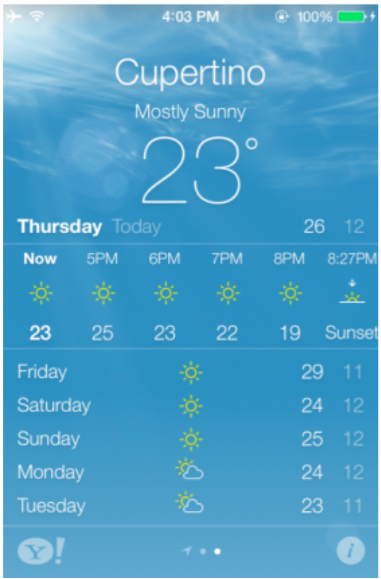
\includegraphics[height = 60 mm ]{images/meteo.png} \\
				\end{figure}

				\textbf{Liste Nelle utility app}: Le \emph{liste} nelle utility app sono in genere \emph{non gerarchicamente collegate}. (Es: Tempo in diverse città.) \\

				\textbf{Preferenze}: Le preferenze sono soggette a frequenti cambiamenti alla configurazione. Rimanendo al nostro esempio sul meteo, vediamo quanto appena detto quando personalizziamo le città di cui vogliamo rimanere informati. Oltre questo, è bene notare che l'utente ha necessità di modificare queste preferenze dall’interno dell’applicazione.

			\subsubsection{Immersive Application} \label{sez:immersiveApp}
				Nelle \emph{Immersive Application}, l'utente si ``immerge'' nell'applicazione, e non presta attenzione all'ambiente circostante. (Richiede una concentrazione continuata. Esempio Classico: Gioco) \\

				Gli ambienti in questo tipo di applicazioni sono \emph{ricchi}, ed a differenza delle \emph{Productivity Application} non conta molto il \emph{task}, ma l'esperienza che ha l'utente. Bisogna dare soddisfazione a quest'ultimo!

				\textbf{Interazione Immersive Application}: Un immersive app non usa dei controlli standard, ma ne usa anche dei propri! Cercare i controlli e scoprirne il funzionamento è parte dell’esperienza di un'immersive application. Quest'ultime inoltre usano spesso grandi quantità di dati, ma li mostrano in modo particolare nel contesto. \\

				Concludiamo con qualche esempio di immersive application. Nel primo, è possibile vedere l'esempio più classico di immersive application, ovvero un \emph{videogioco}.\footnote{Se non conosci worms, sei una brutta persona.}
				\begin{center}
				\begin{figure}[htbp]
				\centering%
				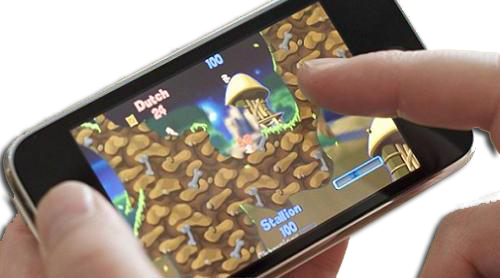
\includegraphics[height = 50mm]{images/worms.png}
				%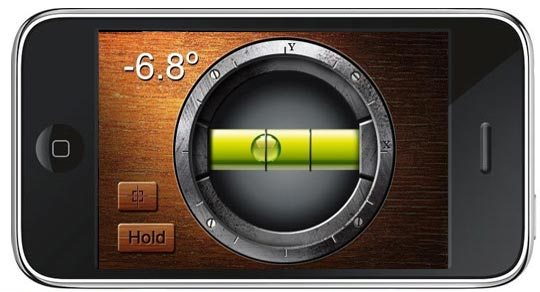
\includegraphics[height = 45mm]{images/livella.jpg}
				\end{figure}
				\end{center}
				In questo secondo esempio invece, è possibile vedere un secondo esempio di immersive app che non è un videogioco, ovvero l'applicazione \emph{``Livella''}:
				\begin{center}
				\begin{figure}[htbp]
				\centering%
				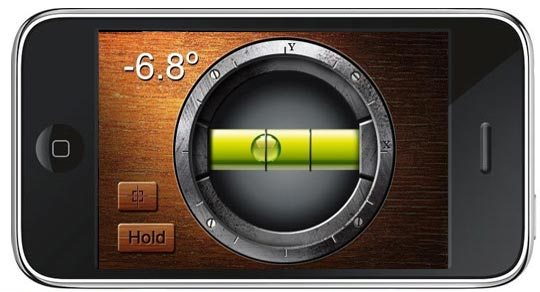
\includegraphics[height = 50mm]{images/livella.jpg}
				\end{figure}
				\end{center}

		\subsection{Principi Per Le Interfacce Mobili} \label{sec:principiPerLeInterfacceMobili}
			Esistono degli elementi comuni a tutte le interfacce mobili, a prescindere che il dispositivo sia \emph{Android}, Apple o altro. Vediamo perciò nel dettaglio quelli più importanti.

			\subsubsection{Metafore} \label{subsec:metafore}
				L’uso di metafore si applica ai sistemi mobili come ai desktop. Esempi: (nell'iPhone)
				\begin{itemize}
				\item Interruttori On/Off
				\item Controlli Play/Pause
				\item Picker (ruote con informazioni)
				\end{itemize}
				Parleremo in maggior dettaglio di questo argomento in futuro. (\ref{sez:metafore})

			\subsubsection{Manipolazione Diretta} \label{sez:manipolazioneDiretta}
				La manipolazione diretta permette agli utenti di controllare qualcosa che altrimenti risulterebbe astratto. È importante che gli oggetti manipolabili siano sempre visibili e che il risultato del gesto sia immediato.

			\subsubsection{Selezionare Invece Di Scrivere} \label{sez:selezionaInveceDiScrivere}
				Sullo smartphone, se possibile, è preferibile utilizzare la selezione tramite l'uso di \emph{liste} piuttosto che l'uso di una tastiera, in quanto si potrebbero riscontrare diverse difficoltà, quali:
				\begin{itemize}
				\item Difficoltà nello scrivere con la tastiera piccola
				\item Difficoltà a scrivere in movimento o di fretta
				\item Difficoltà a ricordare comandi o elenchi di oggetti
				\end{itemize}
				Inoltre, c'è da tener presente che presentare diverse scelte, fa concentrare l’utente sul task anzichè sui comandi dell’applicazione.

			\subsubsection{Feedback} \label{sez:feedback}
				È importante dare dei feedback all'utente a seguito di ogni azione. Il feedback può essere \emph{visuale, uditivo o tattile}, e non è necessariamente unico quando si presenta. \\

				Nel caso di operazioni lunghe inoltre, mostrare il \emph{progresso} è un buon modo per dare qualche feedback all'utente, così come le \emph{animazioni}, che più in generale servono a migliorare \emph{l'user experience}. (E non sono fine a se stesse.)

			\subsubsection{Controllo All'utente} \label{sez:conotrolloUtente}
				Una cosa molto importante riguarda il \emph{controllo} che si da all'utente. Quest'ultimo deve essere in grado di poter \emph{controllare} le azioni che il dispositivo esegue, ed è quindi preferibile chiedere ``conferma'' solo in caso di \emph{azioni distruttive}. (In caso contrario, evitale. Panizzi non a caso ci tiene a questa cosa) \\

				È importante anche permette all'utente di annullare operazioni prima che vengano eseguite, nonché di annullare eventuali operazioni in corso ove possibile.

			\subsubsection{Integrità Estetica} \label{sez:integritaEstetica}
				Misura quanto l’estetica dell’applicazione si integra con la sua funzionalità. Esempi:
				\begin{description}
				\item[Immersive App] Coerenza interna
				\item[Productivity App] Elementi decorativi molto discreti
				\end{description}

	\newpage
	\section{Android}
		\textbf{Nota Bene}: Prima di iniziare questa sezione, è importante aver compreso quanto detto nella precedente sezione ``Principi Per Le Interfacce Mobili''. (\ref{sec:principiPerLeInterfacceMobili})

		\subsection{Concetti Base}
			Nelle interfacce, ci sono alcuni concetti che ormai sono entrati nella quotidianità dell'utente, diventando così dei \emph{standard}. Tra questi, sottolineiamo:
			\begin{description}
			\item[Standard Widgets] Ovvero tutti quei \emph{componenti grafici} che per via del loro utilizzo, sono diventati dei veri e propri \emph{standard.} (Come fa intuire la parola stessa)
			\item[Standard Gestures] I ``gesti'' effettuati sull'interfaccia, che ormai sono consolidati. (Per altre info in merito, consultare la seguente \href{https://www.google.com/design/spec/patterns/gestures.html#}{pagina}.)
			\end{description}

		\subsection{Metafora} \label{sez:metafore}
			Le metafore si usano quando dobbiamo parlare di una cosa per spiegarne un altra.. La filosofia è:
			\begin{center}
			\begin{em}
			Prendi una cosa che conosci dalla vita reale, e usala nell'iterfaccia per far si che sia di facile comprensione.
			\end{em} 
			\end{center}
			Nonostante le metafore siano dunque auto esplicative, da sole a volte non bastano.. quindi, quando è opportuno, è giusto sapere accompagnare quest'ultime con le giuste indicazioni. (Per Esempi di metafore, fare riferimento al precedente paragrafo: \ref{subsec:metafore})

		\subsection{Discoverability} \label{Discoverability}
			La Discoverability, (\emph{``Possibilità Di Scoprire''}) è l'abilità che ha \emph{qualcosa} (nell'interfaccia) di ``farsi trovare''. (Fonti: \href{https://en.wikipedia.org/wiki/Discoverability}{wikipedia})\\
			Se c'è infatti qualcosa che non si vede nella nostra applicazione, è importante farla notare in qualche modo all'utente. \\

			Una cosa molto importante è dunque quella di: \emph{Non nascondere i controlli!} Si possono nascondere dei task secondari, solamente se sono standard. È molto importante che le cose che aggiungiamo siamo dunque \emph{``discoverable''}. 

		\subsection{Action And Reaction}
			In generale, si pretende sempre una reazione da parte del sistema a seguito di un azione. In caso contrario, (come sappiamo tutti) l'assenza di questa reazione potrebbe portare frustrazione/insoddisfazione all'utente.

			\subsubsection{Manipolazione diretta}
				Un esempio in cui necessitiamo avere una reazione a seguito di un azione da parte del sistema, riguarda la 
				\emph{Manipolazione diretta}. (di cui abbiamo già parlato. \ref{sez:manipolazioneDiretta}) Un esempio è quando ad esempio prendiamo e spostiamo un oggetto. Quando faccio queste azioni, voglio che l'app risponda in tempo reale! \emph{Esempio pratico}:
				\begin{figure}[htbp]
				\centering
				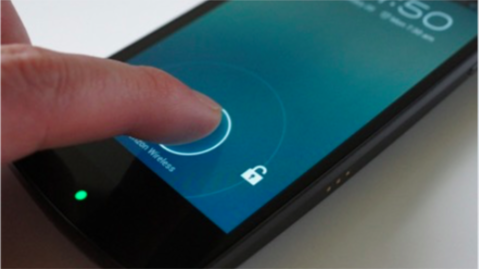
\includegraphics[height = 40mm]{images/sblocco.png}
				\caption{Quando sblocco lo smartphone, Trascino il lock.}
				\end{figure}

		\subsection{Users in Control} \label{ControlloUtente}
			È importante che l'utente abbia sempre il controllo della situazione. (Ne abbiamo già parlato nel paragrafo: \ref{sez:conotrolloUtente}) Su \emph{Android} questo si fa grazie a dei menú, il cui titolo è nella cosidetta \emph{Action Bar}.\\

			\subsubsection{Action Bar} \label{sez:actionBar}
				\emph{Cosa è una action bar?} Una \emph{action bar} è un oggetto presente nella parte superiore di ogni schermata, e che in genere continua ad essere presente in ogni momento in cui usiamo l'app.\footnote{A patto che non sia \emph{immersive}. (\ref{sez:immersiveApp})} Quest'oggetto permette diverse azioni molto importanti, quali:
				\begin{itemize}
				\item Permette di svolgere azioni importanti in maniera molto semplice ed intuitiva.
				\item Supporta navigazioni consistenti e \emph{view switching} tra apps.
				\item Riduce l'ingombro delle azioni meno frequenti.
				\item Provvede a dare un identità all'app grazie all'apposito spazio dedicato.
				\end{itemize}

			\subsubsection{Tasto Back} \label{TastoBackAndroid}
				Il \emph{``back''} come sappiamo, è una funzionalità molto importante, ma su android non è univoca! Infatti abbiamo due tipologie di \emph{back}:
				\begin{itemize}
				\item Il back fisico, che torna sempre all'ultima schermata che abbiamo visualizzato. (stile \emph{stack})
				\item Il back virtuale, che torna alla schermata che sull'albero della progettazione è precedente. Implementare questo secondo tipo di back, spetta però al progettista!\footnote{Di fatto quindi, possiamo dare al back anche un altro significato\dots Nonostante questo, è importante che si segua lo standard per quanto riguarda il back, per non causare inutili confusioni all'utente.}
				\end{itemize}
				
			\subsubsection{Cancel} \label{CancelAndroid}
				Il tasto cancel è sempre presente in un app. Spesso si attribuisce a questo bottone il significato errato di ``cancella'', ma così non è! (infatti è un \emph{false friend}) Questo di fatto interrompere semplicemente l'azione cominciata. (Annulla)

	 		\subsubsection{Barra di progresso} \label{BarraDiProgressoAndroid}
				Necessaria se l'operazione impiega più di quanto l'utente è tollerante ad aspettare. (in genere un secondo) Vediamone le varie tipologie:
				\begin{itemize}
				\item Determinate: ovvero sò quanto manca.
				\item Indeterminate: Non sò quanto manca. (cerchio che gira all'infinito, o barretta che va da una parte all'altra)
				\item Buffer Tipica nei video (mi dice la parte caricata e quella ancora da caricare.)
				\item Query Determinate e Indeterminate
				\end{itemize}
				Per chiarire al meglio i concetti, ecco un esempio autoesplicativo:
				\begin{center}
				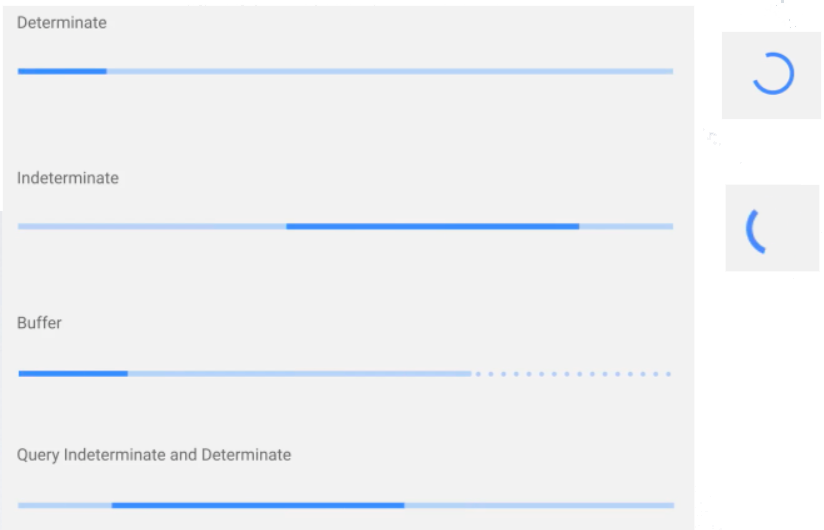
\includegraphics[height = 50 mm]{images/progressBar.png}
				\end{center}

			\subsubsection{Undo}
				Comando che mette l'utente a suo agio, visto che gli permette di rimediare ad eventuali errori. L'unico svantaggio si questo comando, è il fatto che non è semplice dal punto di vista realizzativo.

		\subsection{Customize}

			\subsubsection{Learn People Preferences}
				Ogni utente ripete certe azioni, e queste sono spesso diverse da utente a utente. È importante quindi raccogliere informazioni dall'uso dell'utente, per apprenderne le preferenze. (e di conseguenza aiutarlo con dei futuri \emph{suggerimenti}) \emph{Esempio:}
				\begin{center}
				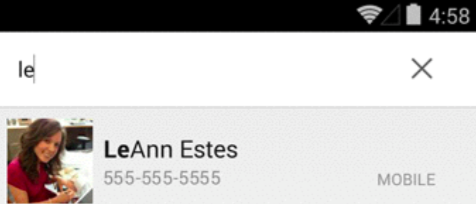
\includegraphics[height = 25mm]{images/suggest.png}
				\end{center}

				\emph{Attenzione!} Questo non và confuso con il suggerimento dato da un ricerca di google ad esempio, dove l'ordine delle cose mostrate rispetta spesso altri criteri.

			\subsubsection{Default}
				Il \emph{Default} riguarda la scelta che verrà presa nel caso in cui l'utente non voglia scegliere. Questa responsabilità sarà presa necessariamente dal designer quando si implementerà l'applicazione. Sta a noi capire qual è l'operazione più gettonata che deve diventare il default per quella determinata azione.

			\subsubsection{Allow Customization}
				Ovviamente bisogna anche permettere all'utente di personalizzare l'ambiente in cui vive. (esempio classico: Personalizzazione sfondo)

		\subsection{Consistency}

			\subsubsection{Same Gesture, Same Action}
				È importante avere \emph{Coerenza} in questa cosa, in quanto vogliamo che ad una determinata azione corrisponda sempre lo stesso comportamento. (Stesse funzioni, stessi widget) \\

				Questa cosa vale anche per il \emph{tema}, che ovviamente non può cambiare da una schermata ad un altra, e che deve quindi \emph{rimanere lo stesso} per \textbf{NON} confondere l'utente. (\textbf{Evita Modi})

		\newpage %Non ce ne è bisogno, ma è meglio prevenire in caso di aggiunte successive.
		\subsection{Material Design} \label{MaterialDesign}
			Il \emph{Material Design} è un \emph{Design Language} sviluppato da Google, che sintetizza i classici principi del buon design con l'innovazione e le possibilità delle nuove tecnologie e della scienza.

			\subsubsection{Principi}
				I principi per quel che riguarda il \emph{Material Design}, (approfondibili \href{https://www.google.com/design/spec/material-design/introduction.html#}{Qui}) sono essenzialmente 3:
				\begin{description}
				\item[Material is the metaphor] I \emph{``Materiali''} sono molto importanti in questo contesto. Questi vengono riproposti nell'interfaccia rispettando i principi della fisica, in modo da dare all'utente un apprendimento più immediato. Vengono esaltati criteri quali \emph{luci}, \emph{Movimenti} e \emph{superfici}, in modo da mettere in risalto il modo in cui gli oggetti interagiscono e siano in relazione tra di loro. (Approfondimenti: \href{https://www.google.com/design/spec/what-is-material/elevation-shadows.html#}{MATERIAL})
				\item[Bold, graphic, intentional] Il modo in cui sono espressi i font, non comportano semplicemente un miglioramento grafico, in quanto creano gerarchie di importanza, \emph{focus} e significati diversi in base al contesto. 
				\item[Motion provides meaning] Quando si effettua un movimento, l'utente si focalizza su quest'ultimo in modo continuato. Bisogna fare in modo che non venga ``stravolto'' l'ambiente circostante, assecondandolo poi con \emph{Feedback} e \emph{Transizioni} quando opportuno.
				\end{description} 

			\subsubsection{Lists \& Cards} \label{sez:listsCardsAndroid}
				Le liste, sono \emph{Items} (omogeni tra di loro) disposti su più linee in un \emph{arrangiamento} verticale, che danno l'impressione di essere un elemento unico. \\

				Gli elenchi basati su \emph{Cards}, sono invece dei pezzi di ``carta'' che contengono dati distinti tra di loro (a differenza dei tipi precedenti). \\

				Per chiarire al meglio questa distinzione, ecco un esempio visivo:
				\begin{figure}[htbp]
				\centering% 
				\subfigure[\protect\url{Lists}\label{fig:list}]%
					{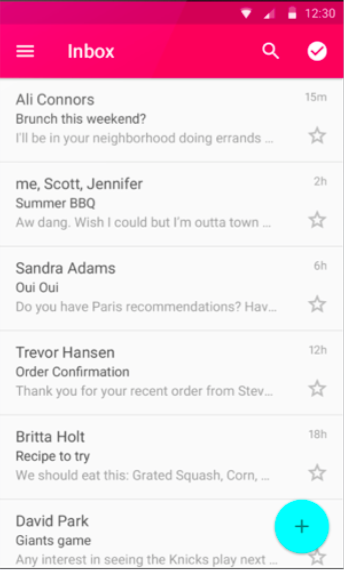
\includegraphics[height = 37 mm]{images/lists.png}}\qquad\qquad 
				\subfigure[\protect\url{Cards}\label{fig:cards}]%
					{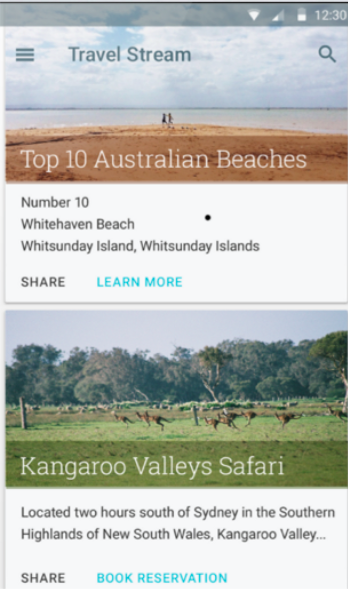
\includegraphics[height = 37 mm]{images/cards.png}}
				\end{figure} 

			\newpage
			\subsubsection{Alerts \& Bottom Sheets} \label{BottomSheetAlertAndroid}
				Gli alert, come sappiamo, sono messaggi di ``allarme'', e sono implementati tramite pop-up o dialogue box. Alcuni sono generati in base alle azioni, mentre altri in maniera asincrona. \\
				\emph{Esempi in base alle azioni}: cancello un elemento, spegnimento, conferma etc. \\

				Questi tipi di alert hanno un nome specifico, e vengono chiamati nel gergo \emph{Bottom Sheets}. \\
				Gli alert ``veri e propri'' invece sono quelli (già accennati) generati in modo \emph{asincrono} dal sistema. Quando vengono attivati, non possiamo fare altre operazioni in quanto entriamo in quello specifico \emph{modo}. \emph{Esempio Alert:} 
				\begin{center}
				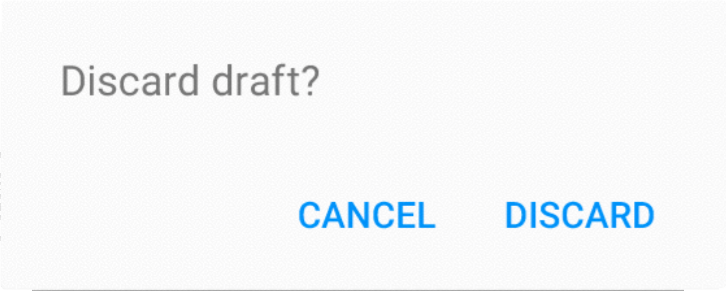
\includegraphics[height = 30mm]{images/alert.png}
				\end{center}
				In questa situazione dunque vogliamo che:
				\begin{itemize}
				\item Venga informato l'utente da situazioni critiche
				\item Vogliamo che l'utente prenda una decisione
				\end{itemize}
				Le bottom sheets invece, presentano una lista di azioni (più dettagliate) possibili. Come abbiamo detto sono ``user solicited'', in quanto seguono una determinata azione eseguita dall'utente. \emph{Esempio:}
				\begin{center}
				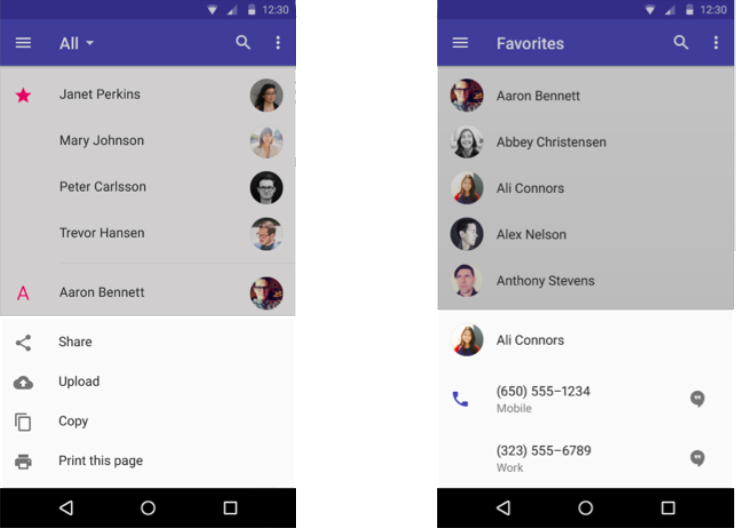
\includegraphics[height = 55mm]{images/bottomSheet.png}
				\end{center}  

	\newpage
	\section{iOS}
		\begin{center}
		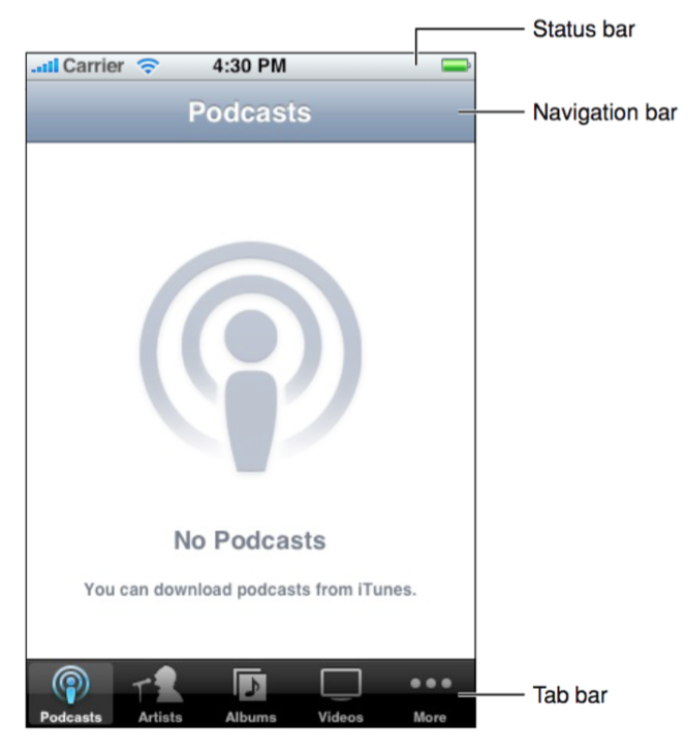
\includegraphics[height = 70mm]{images/varieBariPhone.png}
		\end{center}
		L'interfaccia dell'iphone, si compone da 3 \emph{bar} molto importanti. Analizziamole nel dettaglio	

		\subsection{Navigation Bar} \label{BarIOSApple}
			La navigation bar, ha un duplice scopo. Ovvero quello di:
			\begin{itemize}
			\item Permettere la navigazione attraverso le diverse \emph{viste} dell'applicazione			
			\item Contenere bottoni e altri controlli per gestire gli elementi nella vista
			\end{itemize}
			Vediamone dunque alcune possibili schermate:
			\begin{figure}[htbp]
				\centering% 
				\subfigure[\protect\url{Titolo Della Vista}\label{fig:1}]%
					{
\includegraphics[height = 11 mm]{images/nav1.png}}
				\subfigure[\protect\url{Navigation Control}\label{fig:2}]%
					{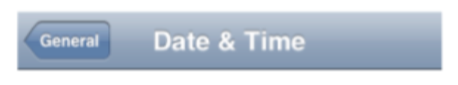
\includegraphics[height = 11 mm]{images/nav2.png}}
				\subfigure[\protect\url{Con Controlli Diversi}\label{fig:3}]%
					{
\includegraphics[height = 9 mm]{images/nav3.png}}
				\subfigure[\protect\url{Misto}\label{fig:4}]%
					{
\includegraphics[height = 9 mm]{images/nav4.png}}
			\end{figure}

		\newpage
		\subsection{Status Bar}
			La \emph{Status Bar} (Barra di stato) serve ad indicare informazioni \emph{rapide} come il livello della batteria e l'ora, ed è presente in quasi in tutte le applicazioni. (ad eccezione delle \emph{immersive application}, dove può essere nascosta) Questa Bar può essere personalizzata nei \emph{colori}, e può mostrare volendo il \emph{network activity indicator.}\footnote{Consigliabile per operazioni più lunghe di un paio di secondi}
			\emph{Esempi Di status bar}:
			\begin{center}
			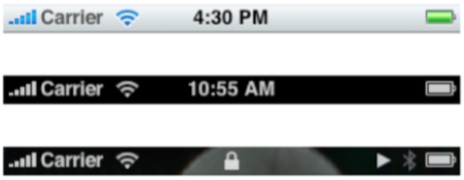
\includegraphics[height = 22mm]{images/statusBar.png}
			\end{center}

		\subsection{Tab Bar} \label{sez:Tabbar}
			La \emph{Tab Bar} permette di gestire diversi \emph{modi}. Essa inoltre:
			\begin{itemize}
			\item Fornisce differenti prospettive sullo stesso insieme di dati
			\item Serve per gestire differenti subtask
			\item Ha ogni tab accessibile da qualunque punto dell’applicazione
			\end{itemize}
			\emph{Esempi:}
			\begin{figure}[htbp]
			\centering%
			\subfigure[\protect\url{App Orologio}\label{fig:tab1}]%
					{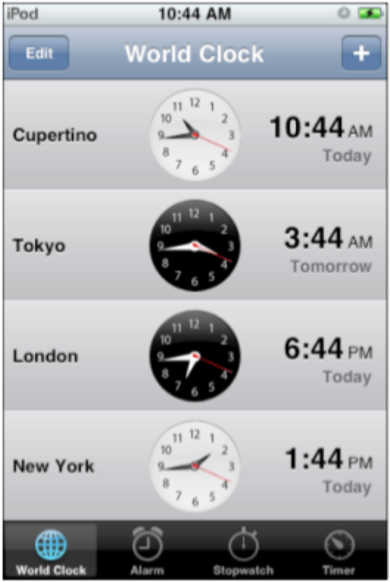
\includegraphics[height = 50 mm]{images/tabBar1.png}}\qquad\qquad
			\subfigure[\protect\url{EsCon+ di 5 icone}\label{fig:tab2}]%
					{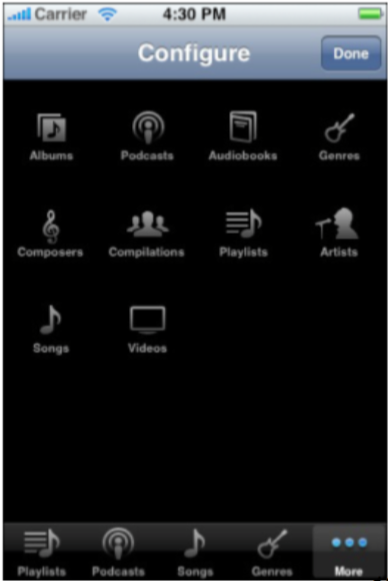
\includegraphics[height = 50 mm]{images/tabBar2.png}}
			\end{figure}
			\\
			È importante osservare come lo standard apple \textbf{imponga} di \emph{non avere} più di 5 icone sulla tab bar, e di come quest'ultime siano personalizzabili a nostro piacimento.\emph{``Mamma Apple''} inoltre, ci dà in merito anche un'altra importante \emph{linea guida}, ovvero che le tab bar (per non disorientare l'utente) o si inseriscono in \emph{tutta l'applicazione}, o \textbf{non} si \emph{inseriscono affatto}. \\

			\emph{Perché devo usare le icone?} Perché una volta che imparo l'azione associata, non dovrò più leggerne il testo associato. (a lungo andare, è molto utile)\\

			Concludendo il paragrafo, è bene notare anche che le icone in questa tipologia di bar, non sono \emph{standard} ma \emph{personalizzabili}.\footnote{Questa è una delle differenze principali che distingue la \emph{tab bar} dalla \emph{tool bar}!} Difatti, quando si usano icone nuove, possiamo \emph{insegnare} l'utente sul significato di quella specifica icona \emph{con del testo}, in modo da permettergli di riconoscerla in futuro. (È sempre meglio eliminare ogni possibile ambiguità con del testo quando si usano icone non standard) 

		\subsection{Toolbar} \label{sez:toolbar}
			\emph{Quando viene visualizzata la Toolbar?} Quando, nel contesto corrente, si possono eseguire più azioni. (va visualizzata in fondo allo schermo) \emph{Esempio:}
			\begin{center}
			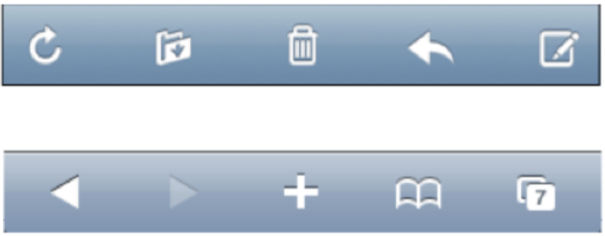
\includegraphics[height = 23mm]{images/toolbar.png}
			\end{center}

			Di fatto quindi, la \emph{toolbar} è una \emph{Barra Strumenti} che contiene dei bottoni/informazioni che servono a gestire il contenuto di una certa vista. Sulle toolbar è importante dire che:
			\begin{itemize}
			\item I bottoni siano equispaziati (Massimo Numero Consentito: 5)
			\item Dimensioni Icona: 44x44 pixel
			\item I bottoni non devono avere il bordo
			\item Non possiamo creare nuove icone. Abbiamo la scelta tra molti bottoni predefiniti\footnote{Perché non possiamo creare nuove icone? Essenzialmente per non disorientare l'utente. Visto che non possiamo tra l'altro inserire testo, avere degli standard predefiniti è, senza dubbio, la scelta migliore.} (al contrario delle tab bar)
			\end{itemize}

		\pagebreak
		\subsection{Alert, Action Sheet e Modal View} \label{sez:ActionSheetModalViewAlert}
			I 3 comandi in questione, hanno la carrateristica che sono \emph{modali}, quindi interrompono il flusso di azioni dell'utente.
			\begin{center}
			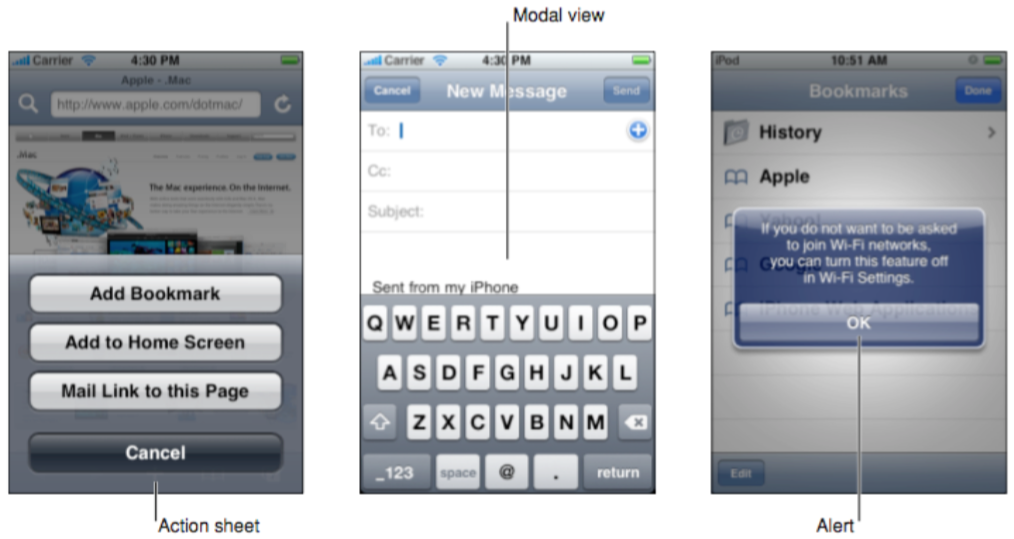
\includegraphics[height = 66mm]{images/actionalert.png}
			\end{center}

			\subsubsection{Alert} \label{sec:alertIphone}
				Come sappiamo dal paragrafo \ref{BottomSheetAlertAndroid}, gli alert forniscono informazioni importanti relative a qualcosa che è accaduto nell’applicazione. Potremmo avere:
				\begin{itemize}
				\item Problemi o cambiamenti della situazione
				\item Problemi inattesi
				\item Richieste per determinate decisioni/Azioni
				\end{itemize}

			\subsubsection{Action Sheet}
				Fornisce opzioni di scelta per l'esecuzione di un azione, ed appare in seguito ad un'azione da parte dell'utente. Queste vengono usate quando ho azioni che:
				\begin{itemize}
				\item Prevedono più possibilità
				\item Sono potenzialmente ``Distruttive''
				\end{itemize}

			\subsubsection{Modal View}
				La \emph{Modal View} offre funzionalità aggiuntive per eseguire un subtask relativo al compito attuale, nascondendo nel frattempo il resto dell'applicazione, rinforzando così l’idea di vista temporanea, modale. (Bottoni ``Fatto'', ``annulla'')

		\subsection{Table View} \label{sez:TableView}
			Il modo in cui vengono visualizzate le tabelle in iOS, varia a seconda della tabella in questione. A differenza di \emph{Android}, qui non ci sono le card, ma 2 diverse tipologie di tabelle. Ovvero:
			\begin{description}
			\item[Plain Table] Equivalgono alle liste su android. c'è una \emph{omogeneità} tra un elemento e l'altro. Possono essere anche indicizzate.
			\item[Grouped Table] I vari elementi sono \emph{raggruppati} in vari gruppi. Ogni ``gruppetto'' ha un \emph{titolo} e un \emph{footer}.
			\end{description}
			Per avere un altro (ed ultimo) esempio grafico di quanto detto, abbiamo un esempio di \emph{Plain Table} (img 1 e 2) e di {Grouped Table}:
			\begin{center}
			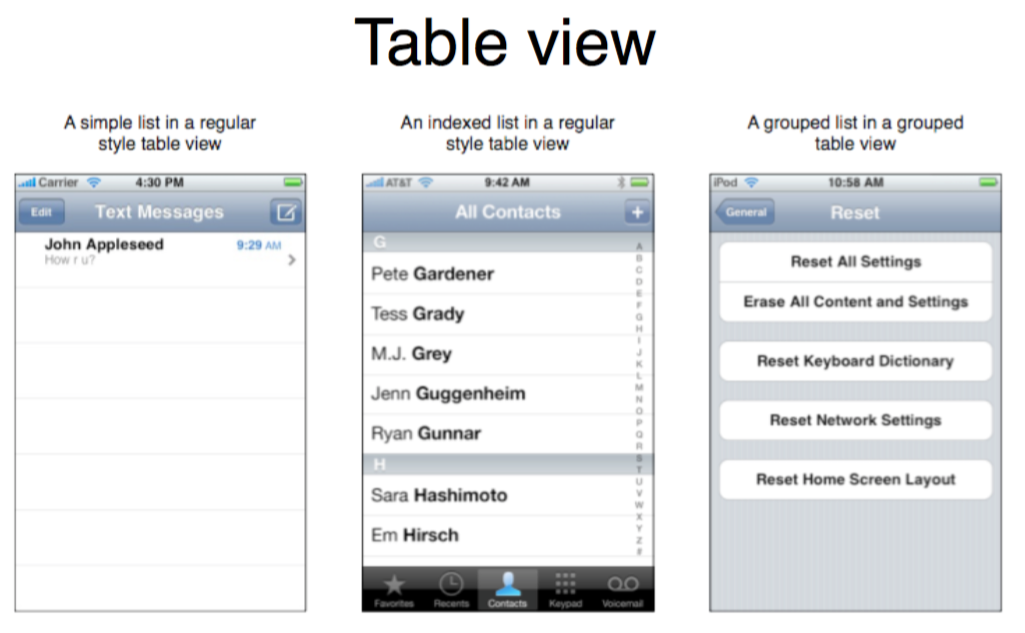
\includegraphics[height = 75mm]{images/tableview.png}
			\end{center}
			\subsubsection{Conclusione}
			Come per \emph{Android}, se si vuole approfondire qualche argomento, è possibile farlo consultando la \href{https://developer.apple.com/library/ios/navigation/}{iOS Developer Library}.
		

\chapter{Domande Esame}
	In questo capitolo finale, verranno elencati esempi di domande (con opportuni riferimenti) chieste dal \emph{prof} in sede di esame, nonché la relazione del \href{https://alexflyce.files.wordpress.com/2016/02/progetto.pdf}{Progetto} del mio gruppo.
	\begin{description}
	\item[Descrivere gli esperimenti between/within groups.] (\ref{sez:wbgroups})
	\item[In che cosa consiste la tecnica del Mago di Oz.] (\ref{sec:Oz})
	\item[Descrivere i cicli iterativi nell'agile UCD.] (\ref{sec:UCD})
	\item[Differenza tra test in laboratorio e test sul campo.] (\ref{sec:laboratoriocampo})
	\item[Che cos`è una tab bar?] (\ref{sez:Tabbar})
	\item[Uso delle metafore: in iOS posso utilizare qualsiasi icona?] No. La cosa varia a seconda della \emph{bar}.
	(Tab bar: \ref{sez:Tabbar} - Toolbar: \ref{sez:toolbar})
	\item[Elencare i vari tipi di tabelle studiati] (\ref{sez:TableView})
	\item[Che cos'è il luogo dell'attenzione e la differenza tra focus e locus.] (\ref{sec:luogoAttenzione})
	\item[Noun Verb - Verb Noun : definizione ed esempi.] (\ref{sec:nounverb})
	\item[Quale stile crea un modo: Noun Verb o Verb Noun? perché?] (\ref{sec:nounverb})
	\item[Analisi Euristica] (\ref{sec:heuristic})
	\item[Alert, Action Sheet, Modal View.] (\ref{sez:ActionSheetModalViewAlert})
	\item[Cosa significa lasciare il controllo all'utente] (\ref{ControlloUtente})
	\item[Descrivere il paper prototyping.] (\ref{sez:PaperPrototyping})
	\item[Perché è preferibili la selezione, rispetto alla scrittura?] (\ref{sez:selezionaInveceDiScrivere})
	\item[Test di usabilità di un prototipo Cartaceo.] (\ref{sez:PaperPrototyping})
	\item[Elencare i vari tipi di ruoli. (administrator, observer etc.)] (\ref{MetodiDiOsservazione})
	\item[Come si può sfruttare il lugo dell'attenzione nel design?] (\ref{sec:luogoAttenzione})
	\item[Differenze interfaccia android/apple.] Ci sono molte differenze tra queste due interfacce:
		\begin{enumerate}
		\item Tipi Di Bar (Action Bar Android: (\ref{sez:actionBar}) - Varie Bar iOS: (\ref{BarIOSApple}))
		\item Tasto Back (\ref{TastoBackAndroid}) (in iOS, il back fisico è inesistente)
		\item Discoverability tasto menu-back Android (\ref{Discoverability}) (in iOS, non ci sono)
		\item Material Design (\ref{MaterialDesign})
		\item Card \& List (\ref{sez:listsCardsAndroid}) VS Table View (\ref{sez:TableView})
		\item Bottom sheet (\ref{BottomSheetAlertAndroid}) VS Action Sheet, Modal View (\ref{sez:ActionSheetModalViewAlert})
		\end{enumerate}
	\item[Differenza Lists e Card Nell'interfaccia Android] (\ref{sez:listsCardsAndroid})
	\item[Descrivi il concetto di ``Discoverability''] (\ref{Discoverability})
	\item[Cos'è un abitudine?] Serie di task effettuati senza necessità di concentrarsi su ciò che si fa. (\ref{sec:abitudine})
	\item[Nelle interviste alcune domande potrebbero essere poste male. Perché?] 
		I principali motivi per cui una domanda potrebbe essere mal posta, sono:
		\begin{enumerate}
			\item Le domande potrebbero contenere all'interno la stessa risposta
			\item Potrebbero essere ambigue/non chiare
			\item Troppo lunghe
			\item Richiedere funzionalità aggiuntive (le cosidette funzionalità \emph{regalate}. Es: ``Ti piacerebbe farti fare il caffè da un app per la salvaguardia ambientale del burika faso?'')
			\item Essere del tipo: ``quante volte hai fatto questo?''
		\end{enumerate}
		Riferimento: \ref{Interviste}.
	\end{description}

\chapter{Conclusione}
	Spero che il pdf vi sia servito e sia stato di vostro gradimento! 
\includegraphics[height = 3mm]{images/smile.png} \\

	Per la segnalazione di errori (o comunicazione), scrivetemi pure alla mia email: \mail{alessandrofrancucci@hotmail.it}, o, se preferite, sul mio profilo \href{https://www.facebook.com/FlyceAlex}{Facebook}. :) \\

	%Se volete invece consultare altri miei lavori/appunti scritti in \LaTeX{}, vi basta visitare la mia pagina \href{https://alexflyce.wordpress.com/}{WordPress}. \\

	\textbf{Concludendo}, se questo pdf vi è stato di aiuto, potete esprimermi la vostra gratitudine tramite una libera donazione con \href{https://www.paypal.me/alexflyce}{\textbf{PayPal Me}}! Ve ne sari molto riconoscente! Anche il semplice gesto di donarmi quanto basta per \emph{un caffè}, mi farebbe capire che tutto il lavoro fatto è stato in qualche modo apprezzato. :') \\

	Detto questo, \emph{Buona fortuna a tutti per l'esame!}

\end{document}